% !TEX program = pdflatex
\documentclass[11pt,letterpaper]{article}

% Packages
\usepackage[utf8]{inputenc}
\usepackage[margin=1in]{geometry}
\usepackage{graphicx}
\usepackage{amsmath}
\usepackage{amssymb}
\usepackage{booktabs}
\usepackage{longtable}
\usepackage{array}
\usepackage{enumitem}
\usepackage{hyperref}
\usepackage{xcolor}
\usepackage{tikz}
\usetikzlibrary{shapes,arrows,positioning,fit,backgrounds}
\usepackage{listings}
\usepackage{fancyhdr}
\usepackage{float}

% Page style
\pagestyle{fancy}
\fancyhf{}
\rhead{Adaptive Learning System Architecture}
\lhead{Principal AI Architecture Plan}
\rfoot{Page \thepage}

% Title information
\title{\textbf{Adaptive Learning System Architecture:\\Evidence-Backed Roadmap for Scale}}
\author{Principal AI Architecture Team}
\date{\today}

% Custom commands
\newcommand{\milestone}[1]{\textbf{#1}}
\newcommand{\metric}[1]{\texttt{#1}}

\begin{document}

\maketitle

\begin{abstract}
This document presents a comprehensive, incremental architecture for an adaptive learning system designed to serve millions of higher education learners. The system delivers micro-learning resources (short video clips and PDF segments) in response to student questions, provides formative assessments, and measures learning gains over time. We compare four architectural approaches, recommend a hybrid RAG-first strategy with bandit-based optimization, and provide a detailed 12-week implementation roadmap with concrete metrics, risks, and mitigation strategies. The architecture prioritizes measurable learning outcomes over engagement metrics and maintains agility for foundation model upgrades.
\end{abstract}

\tableofcontents
\newpage

\section{Executive Summary}

\subsection{Chosen Approach and Rationale}

\begin{itemize}[leftmargin=*]
\item \textbf{Recommended Architecture:} RAG-first with cross-encoder reranking, agentic orchestration, and contextual bandits for content selection, augmented with task-specific LoRA fine-tuning for pedagogical components.

\item \textbf{Why This Beats Alternatives:} Addresses cold-start problem for content recommendation (no historical labels), leverages existing Q\&A/assessment data, enables rapid iteration, maintains model-agnostic flexibility, and provides clear pathway from baseline to optimized system.

\item \textbf{Cold-Start Strategy:} Start with metadata-driven heuristics and semantic similarity (no ML needed), rapidly collect preference data through teacher-in-the-loop and implicit feedback, bootstrap bandit policies within 4--6 weeks.

\item \textbf{Minimality Enforcement:} Hard constraints on resource duration/length, explicit sufficiency scoring (semantic coverage per unit time/pages), segment-level retrieval instead of whole assets, MMR diversification to avoid redundancy.

\item \textbf{Learning Measurement:} IRT-based ability estimation ($\theta$), calibrated item parameters (discrimination $a$, difficulty $b$), longitudinal $\Delta\theta$ tracking, normalized gain metrics that distinguish learning from engagement (time-on-task, clicks).

\item \textbf{Pedagogical Quality:} Few-shot prompted question generation aligned to Bloom taxonomy levels, rubric-based grading with reference answers, distractor quality checks, hint generation, worked examples for scaffolding.

\item \textbf{Data Flywheel:} Existing Q\&A logs seed question generation models, assessment data calibrates difficulty estimators, user interactions train bandit policies, teacher feedback refines retrieval quality through active learning.

\item \textbf{Risk Mitigation:} Retrieval-grounded generation to reduce hallucinations, answerability checks before question generation, refusal paths for out-of-scope queries, privacy-preserving logging, drift detection for item parameters.

\item \textbf{Agility Preserved:} LoRA adapters (not full fine-tuning) for pedagogical tasks, modular architecture allows component swaps, evaluation harness enables A/B testing of model upgrades, prompt libraries versioned alongside models.

\item \textbf{Team Fit:} Leverages agentic AI expertise for orchestration, data science skills for IRT calibration and bandit tuning, avoids heavy ML engineering burden (no custom training infrastructure), uses standard RAG tooling and off-the-shelf LLMs.
\end{itemize}

\newpage

\section{Architecture Options Comparison}

We evaluate four architectural approaches across key dimensions relevant to our constraints and team capabilities.

\subsection{Option A: RAG-First + Reranking + Agentic Orchestration}

\textbf{Components:}
\begin{itemize}
\item Bi-encoder (dense) + BM25 (sparse) hybrid retrieval over chunked content corpus
\item Cross-encoder reranker for top-k candidates
\item MMR (Maximal Marginal Relevance) for diversity
\item LLM-based agentic planner: query understanding $\rightarrow$ retrieval $\rightarrow$ content selection $\rightarrow$ pedagogy tools $\rightarrow$ evaluation $\rightarrow$ next-action
\item Prompt engineering for question generation, grading, hint provision
\end{itemize}

\textbf{Infrastructure:}
\begin{itemize}
\item Vector database (Pinecone, Weaviate, or Qdrant): \$500--\$2k/month at prototype scale
\item LLM API (GPT-4o, Claude Sonnet, Gemini): \$0.01--0.03/1k tokens
\item Embedding API (OpenAI text-embedding-3, Cohere): \$0.0001--0.0002/1k tokens
\item Cross-encoder inference (can self-host small models like ms-marco-MiniLM-L-12)
\end{itemize}

\textbf{Cost Estimate (10k learners, 5 interactions/day):}
\begin{itemize}
\item Embeddings: $\sim$\$50/month
\item LLM calls: $\sim$\$1,500--\$3,000/month
\item Vector DB: $\sim$\$500--\$1,000/month
\item Total: \$2,000--\$4,500/month at prototype scale
\end{itemize}

\textbf{Latency:}
\begin{itemize}
\item Retrieval (hybrid + rerank): 200--500ms
\item LLM generation (streaming): 1--3s to first token, 3--8s total
\item End-to-end: 4--10s for full interaction
\end{itemize}

\textbf{Data Needs:}
\begin{itemize}
\item Minimal for cold-start: content corpus only
\item No labeled training data required
\item Can start immediately with existing materials
\end{itemize}

\textbf{Expected Quality:}
\begin{itemize}
\item Retrieval: 70--85\% Recall@10 with hybrid search
\item Question quality: 60--75\% expert approval (prompt-only)
\item Minimality: Depends on prompting and post-processing
\item Learning gains: Baseline to improve upon
\end{itemize}

\textbf{Cold-Start Viability:} \textcolor{green}{Excellent} -- Works day-one with zero historical labels

\textbf{Expected Learning Impact:} Moderate (depends on content quality and prompt engineering)

\textbf{Team Fit:} \textcolor{green}{Excellent} -- Matches agentic AI expertise, no ML training required

\textbf{Risks:}
\begin{itemize}
\item Prompt brittleness across domains
\item No learning from user feedback (static)
\item Hallucination risk if retrieval fails
\item Cost scales linearly with usage
\end{itemize}

\subsection{Option B: Lightweight Fine-Tuning (LoRA/PEFT) + RAG}

\textbf{Components:}
\begin{itemize}
\item Same RAG stack as Option A
\item LoRA adapters for: (1) question generation, (2) rubric-based grading, (3) distractor generation, (4) pedagogical style (hints, explanations)
\item Base models: Llama 3.1 70B, Mistral Large, or GPT-4o
\item Adapter inference via vLLM or Lorax for efficient serving
\end{itemize}

\textbf{Infrastructure:}
\begin{itemize}
\item Same vector DB as Option A
\item LoRA training: 1--2x A100 GPUs for 4--12 hours per adapter (\$50--\$200/training run on cloud)
\item Inference: Self-hosted vLLM on 2--4x A100s or API with adapters
\item Storage for adapters: $<$1GB per adapter
\end{itemize}

\textbf{Cost Estimate:}
\begin{itemize}
\item Training: \$500--\$1,500 one-time per adapter (4 adapters $\rightarrow$ \$2k--\$6k)
\item Inference (self-hosted): \$2,000--\$4,000/month GPU costs
\item OR API + adapters: Similar to Option A + adapter overhead
\item Total: \$2,500--\$5,000/month ongoing
\end{itemize}

\textbf{Latency:}
\begin{itemize}
\item Similar to Option A (adapter adds $<$50ms)
\item Self-hosting can reduce latency by 500--1000ms vs. API
\end{itemize}

\textbf{Data Needs:}
\begin{itemize}
\item Minimum 500--2,000 high-quality examples per task
\item Existing Q\&A/assessment logs provide seed data for question generation and grading
\item Need manual labeling for distractor quality and pedagogical style (1--2 weeks of expert time)
\end{itemize}

\textbf{Expected Quality:}
\begin{itemize}
\item Question quality: 75--90\% expert approval (10--15\% boost over prompting)
\item Grading consistency: 85--95\% agreement with human rubrics
\item Distractor quality: Significant improvement in plausibility
\item Learning gains: 5--15\% improvement over prompt-only baseline (estimated)
\end{itemize}

\textbf{Cold-Start Viability:} \textcolor{orange}{Moderate} -- Requires 2--4 weeks for data collection + training

\textbf{Expected Learning Impact:} High (task-specific optimization improves pedagogical quality)

\textbf{Team Fit:} \textcolor{green}{Good} -- Data scientists can handle LoRA training, less complex than full FT

\textbf{Risks:}
\begin{itemize}
\item Adapter drift when base models update
\item Need retraining cadence (every 6--12 months)
\item Overfitting if training data not diverse enough
\item Inference complexity (managing multiple adapters)
\end{itemize}

\subsection{Option C: RL/Bandits for Content Selection + RAG Baseline}

\textbf{Components:}
\begin{itemize}
\item Option A (RAG-first) as baseline retrieval and pedagogy
\item Contextual bandit layer on top: learns which content chunks maximize learning + minimality
\item Context: student ability $\theta$, query embedding, prior performance, resource metadata
\item Actions: select from top-k retrieved candidates
\item Reward: $R = w_1 \cdot \Delta\theta + w_2 \cdot \text{brevity} - w_3 \cdot \text{irrelevance}$
\item Start with Thompson Sampling or UCB, graduate to offline RL if sufficient data
\end{itemize}

\textbf{Infrastructure:}
\begin{itemize}
\item Same as Option A for RAG
\item Bandit policy server: lightweight (Redis + Python service)
\item Logging infrastructure: event stream (Kafka/Kinesis) + data warehouse
\item Offline evaluation: IPS/DR estimators, simulator for policy testing
\end{itemize}

\textbf{Cost Estimate:}
\begin{itemize}
\item Incremental over Option A: \$200--\$500/month for bandit infra
\item Data storage/processing: \$100--\$300/month
\item Total: \$2,300--\$5,000/month
\end{itemize}

\textbf{Latency:}
\begin{itemize}
\item Policy inference: $<$50ms (table lookup or simple model)
\item Total latency: Same as Option A + 50ms
\end{itemize}

\textbf{Data Needs:}
\begin{itemize}
\item Cold-start: Can use uniform random or heuristic policy for 2--4 weeks
\item Training data: Needs 10k--50k logged interactions before policy improves over heuristics
\item Continuous feedback loop essential
\end{itemize}

\textbf{Expected Quality:}
\begin{itemize}
\item Retrieval/selection: 10--25\% improvement over static ranking after sufficient data
\item Minimality: Direct optimization via reward leads to 15--30\% shorter resources
\item Learning gains: 10--20\% improvement over non-personalized baseline (after convergence)
\end{itemize}

\textbf{Cold-Start Viability:} \textcolor{orange}{Moderate} -- Starts with heuristics, improves over 4--8 weeks

\textbf{Expected Learning Impact:} Very High (directly optimizes for learning outcomes)

\textbf{Team Fit:} \textcolor{green}{Good} -- Data scientists have expertise; bandit theory is mature

\textbf{Risks:}
\begin{itemize}
\item Delayed reward signal (learning happens over days/weeks)
\item Need careful reward design to avoid gaming (e.g., always selecting shortest resources)
\item Off-policy evaluation is noisy; need large sample sizes
\item Safety constraints (prevent over-exploration of bad content)
\end{itemize}

\subsection{Option D: Fully Fine-Tuned Task-Specific Models}

\textbf{Components:}
\begin{itemize}
\item Small, specialized models (1--13B parameters) fully fine-tuned for each task
\item Question generator: Llama 3.1 8B fine-tuned on 10k+ exemplars
\item Grader: T5-XXL fine-tuned on rubric-scored responses
\item Distractor generator: GPT-2 or Llama 7B fine-tuned
\item Content selector: Cross-encoder fine-tuned on relevance labels
\item RAG uses standard retrieval (no fine-tuning)
\end{itemize}

\textbf{Infrastructure:}
\begin{itemize}
\item Training: 4--8x A100s for 1--3 days per model (\$500--\$2,000/model)
\item Inference: Self-hosted on 2--4x GPUs or use smaller models on CPU
\item Model storage: 5--50GB per model
\end{itemize}

\textbf{Cost Estimate:}
\begin{itemize}
\item Training: \$2,000--\$8,000 one-time (4 models)
\item Inference: \$1,500--\$3,000/month (self-hosted) or \$500--\$1,000/month (small models)
\item Total: \$1,500--\$3,000/month ongoing
\end{itemize}

\textbf{Latency:}
\begin{itemize}
\item Small models: 100--500ms per task
\item Can pipeline tasks in parallel
\item Total: 2--5s (faster than large LLM)
\end{itemize}

\textbf{Data Needs:}
\begin{itemize}
\item Highest data requirements: 10k--50k examples per task
\item Months of manual labeling effort
\item Existing Q\&A logs insufficient without heavy curation
\end{itemize}

\textbf{Expected Quality:}
\begin{itemize}
\item Potentially highest quality for specific tasks (90--95\% on benchmarks)
\item Consistency and reliability superior to prompting
\item But: brittle to domain shifts, requires retraining for new content types
\end{itemize}

\textbf{Cold-Start Viability:} \textcolor{red}{Poor} -- Requires 2--6 months of data collection + training

\textbf{Expected Learning Impact:} High (once trained), but delayed

\textbf{Team Fit:} \textcolor{orange}{Moderate} -- Requires ML engineering, GPU infrastructure, complex training pipelines

\textbf{Risks:}
\begin{itemize}
\item Long time-to-value (3--6 months before deployment)
\item Model maintenance burden (multiple models to version and monitor)
\item Overfitting to training distribution
\item Difficult to iterate (retraining is slow and expensive)
\item Loss of flexibility as foundation models improve
\end{itemize}

\subsection{Comparison Table}

\begin{table}[H]
\centering
\small
\begin{tabular}{@{}p{2.5cm}p{2.3cm}p{2.3cm}p{2.3cm}p{2.3cm}p{2.3cm}@{}}
\toprule
\textbf{Dimension} & \textbf{Option A: RAG-First} & \textbf{Option B: LoRA+RAG} & \textbf{Option C: Bandits+RAG} & \textbf{Option D: Full FT} \\
\midrule
\textbf{Monthly Cost} & \$2k--\$4.5k & \$2.5k--\$5k & \$2.3k--\$5k & \$1.5k--\$3k \\
\textbf{Latency} & 4--10s & 4--10s & 4--10s & 2--5s \\
\textbf{Data Needs} & None (zero-shot) & 0.5k--2k per task & 10k--50k interactions & 10k--50k per task \\
\textbf{Time to Deploy} & 1--2 weeks & 4--6 weeks & 2 weeks (baseline) + 6--8 weeks (optimized) & 3--6 months \\
\textbf{Cold-Start Viability} & Excellent & Moderate & Moderate & Poor \\
\textbf{Learning Impact} & Baseline (60--70\%) & High (75--85\%) & Very High (80--90\%) & High (85--95\%, delayed) \\
\textbf{Team Fit} & Excellent & Good & Good & Moderate \\
\textbf{Agility} & High (prompt changes only) & High (swap adapters) & Moderate (policy updates) & Low (retrain required) \\
\textbf{Scalability} & Linear API costs & GPU costs + some API & Similar to A + bandit overhead & Self-hosted, lower marginal cost \\
\textbf{Risks} & Hallucinations, prompt drift & Adapter-model mismatch & Reward design, delayed feedback & Long dev cycle, brittleness \\
\bottomrule
\end{tabular}
\caption{Architecture Options Comparison}
\label{tab:arch-compare}
\end{table}

\subsection{Recommendation}

\textbf{Start with Option A (RAG-First), evolve to hybrid A+C (Bandits), selectively add B (LoRA) for pedagogy.}

\textbf{Rationale:}
\begin{enumerate}
\item \textbf{Cold-start imperative:} We have no historical content recommendation labels. Option A works immediately.
\item \textbf{Rapid learning:} Option C (bandits) can start collecting data from day one on top of Option A baseline.
\item \textbf{Strategic fine-tuning:} Option B (LoRA) addresses pedagogical quality after we validate baseline retrieval works.
\item \textbf{Avoid premature optimization:} Option D locks us into brittle, expensive models before we understand the problem.
\item \textbf{Agility:} A+B+C keeps us model-agnostic and able to upgrade foundation models.
\end{enumerate}

\newpage

\section{Final Recommended Architecture}

\subsection{System Overview}

The recommended architecture is a modular, layered system that combines:
\begin{enumerate}
\item \textbf{Hybrid Retrieval Layer:} BM25 + dense embeddings with cross-encoder reranking
\item \textbf{Content Minimization Layer:} Segment detection, sufficiency scoring, length constraints
\item \textbf{Pedagogical Layer:} Question generation, rubric grading, hint provision, worked examples
\item \textbf{Assessment \& Analytics:} IRT-based ability estimation, item calibration, learning gain tracking
\item \textbf{Agentic Orchestration:} Multi-step planner coordinating retrieval, selection, pedagogy, evaluation
\item \textbf{Bandit Optimization:} Contextual bandits for content selection under multi-objective reward
\end{enumerate}

\subsection{Architecture Diagram}

\begin{figure}[H]
\centering
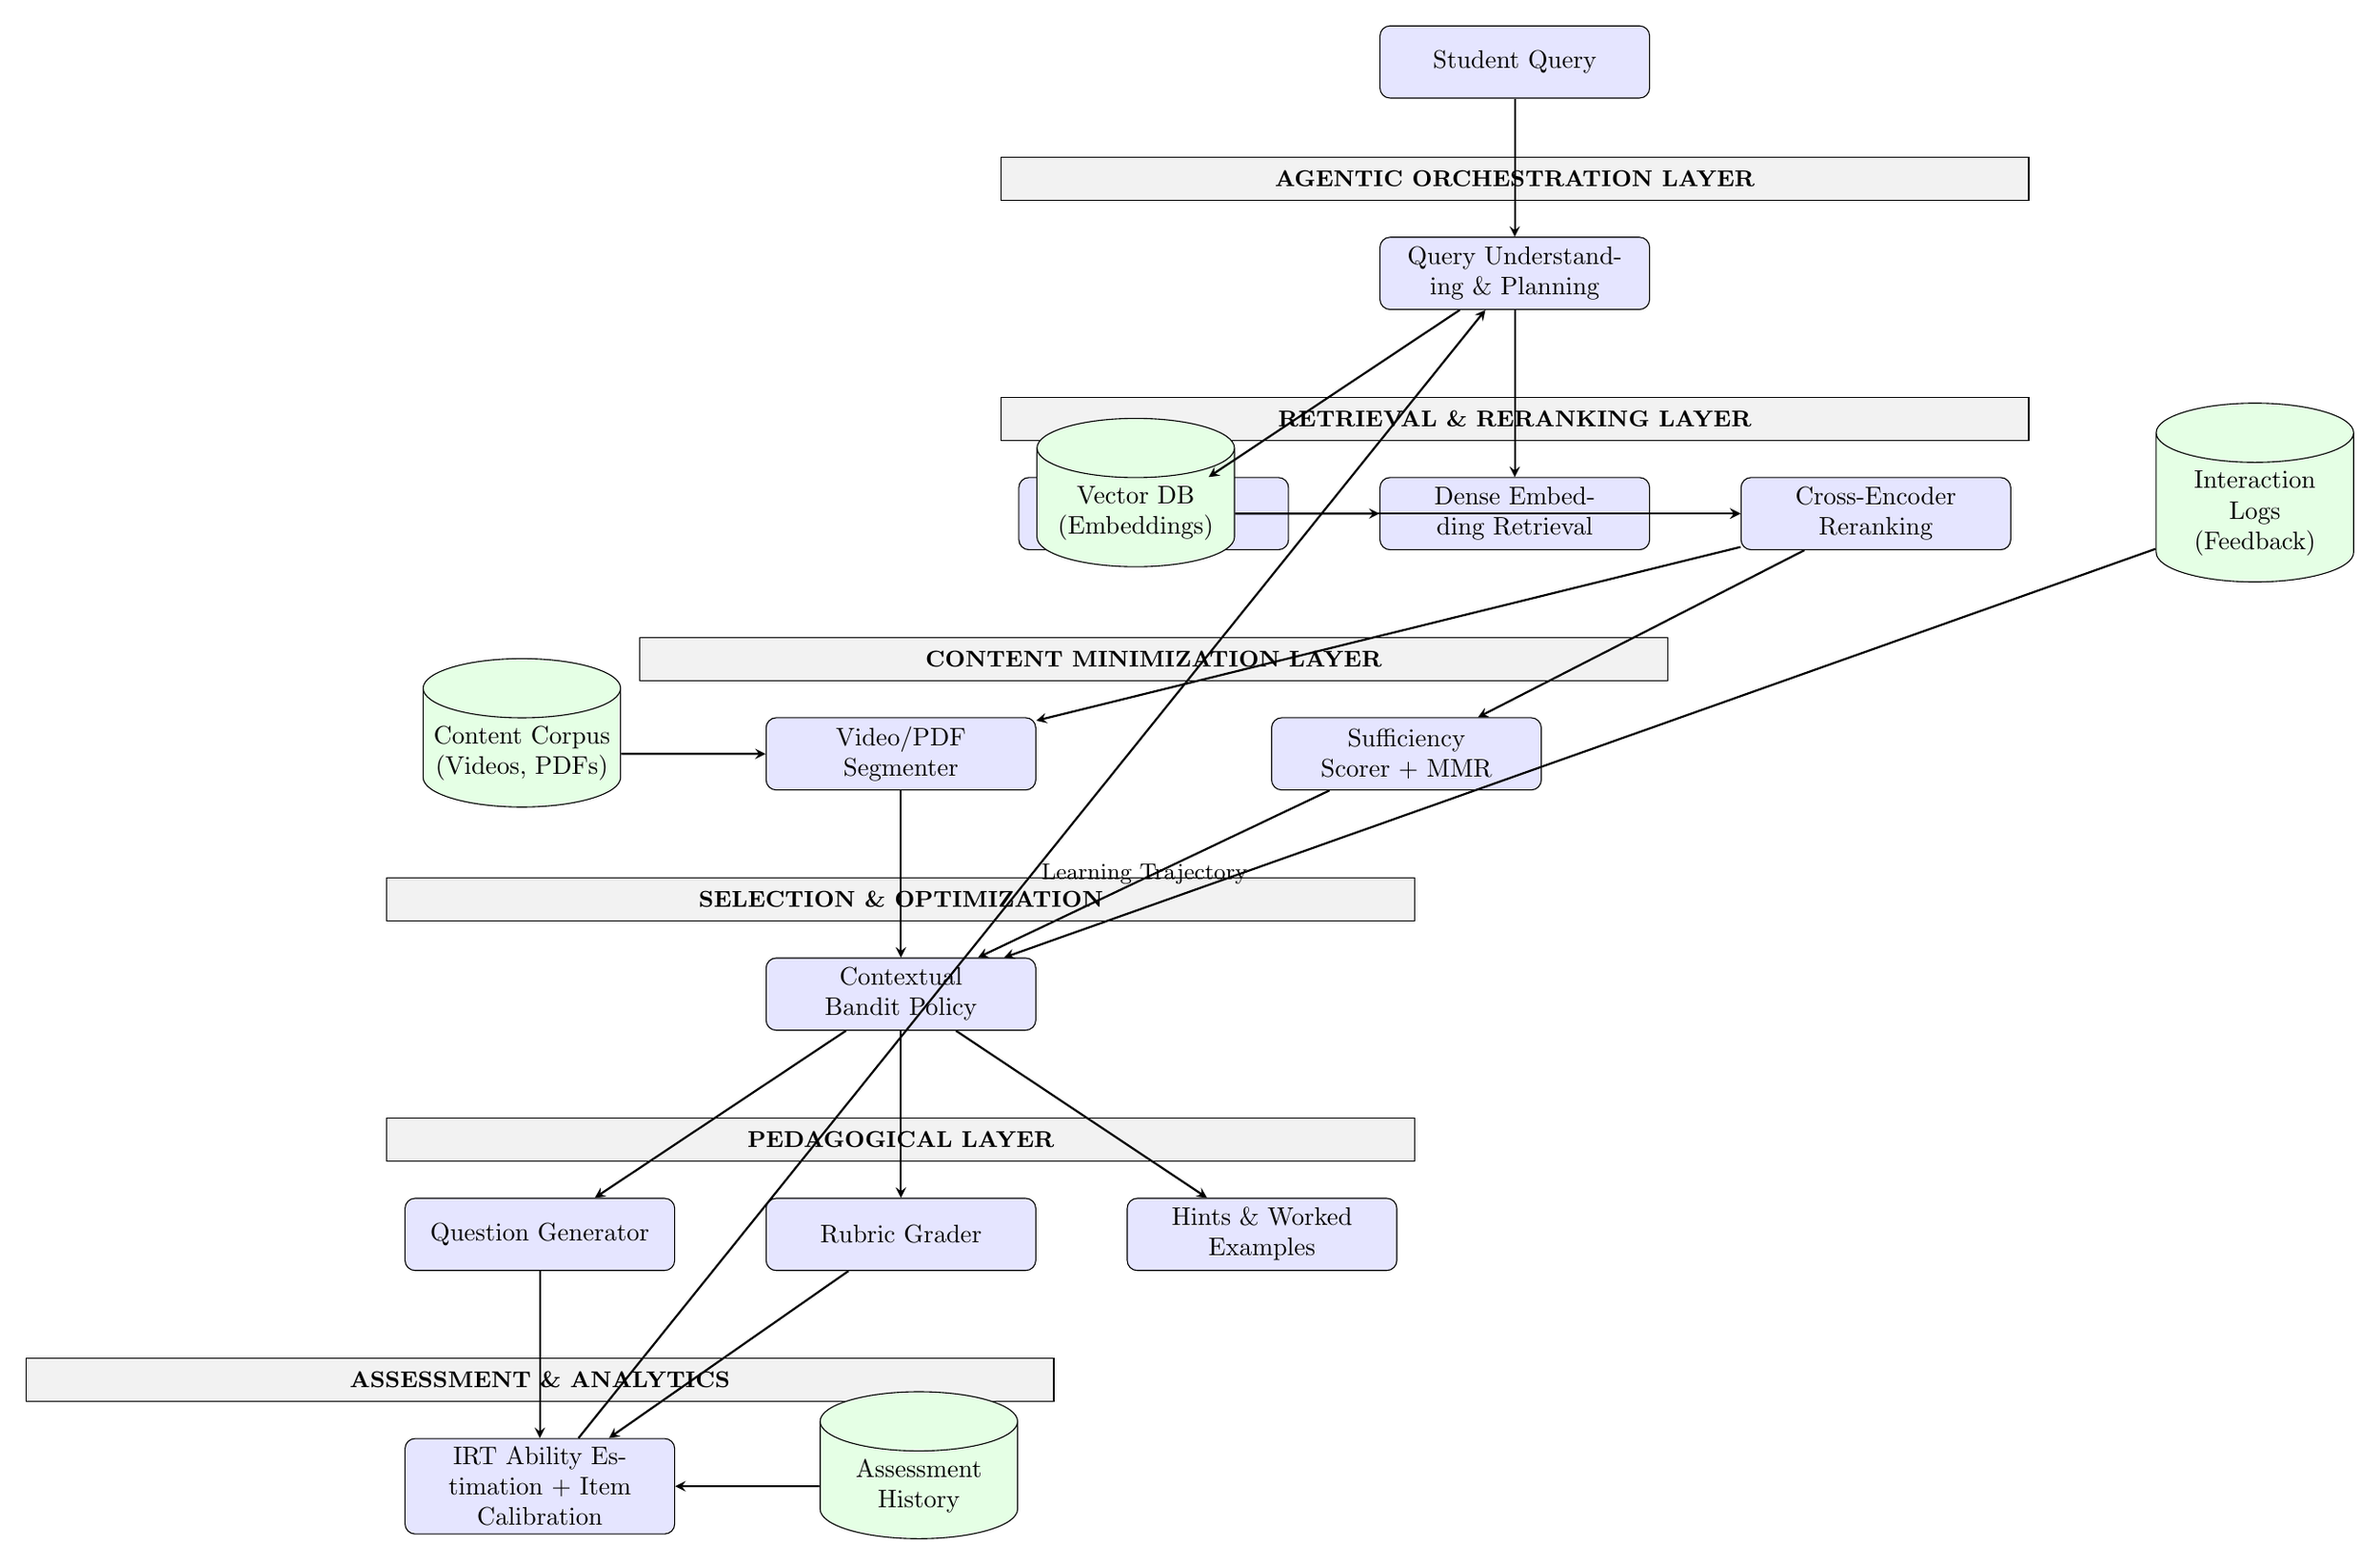
\begin{tikzpicture}[
    node distance=0.8cm and 1cm,
    component/.style={rectangle, draw, fill=blue!10, text width=3.5cm, text centered, minimum height=1cm, rounded corners},
    layer/.style={rectangle, draw, fill=gray!10, text width=14cm, text centered, minimum height=0.6cm, font=\small\bfseries},
    data/.style={cylinder, draw, fill=green!10, text width=2.5cm, text centered, minimum height=0.8cm, aspect=0.3, shape border rotate=90},
    arrow/.style={->, >=stealth, thick}
]

% User interaction
\node[component] (user) {Student Query};

% Agentic orchestration layer
\node[layer, below=of user] (agent-layer) {AGENTIC ORCHESTRATION LAYER};
\node[component, below=0.5cm of agent-layer] (planner) {Query Understanding \& Planning};

% Retrieval layer
\node[layer, below=1.2cm of planner] (retrieval-layer) {RETRIEVAL \& RERANKING LAYER};
\node[component, below=0.5cm of retrieval-layer, xshift=-5cm] (bm25) {BM25 Sparse Retrieval};
\node[component, below=0.5cm of retrieval-layer, xshift=0cm] (dense) {Dense Embedding Retrieval};
\node[component, below=0.5cm of retrieval-layer, xshift=5cm] (reranker) {Cross-Encoder Reranking};

% Content minimization
\node[layer, below=1.2cm of bm25] (content-layer) {CONTENT MINIMIZATION LAYER};
\node[component, below=0.5cm of content-layer, xshift=-3.5cm] (segmenter) {Video/PDF Segmenter};
\node[component, below=0.5cm of content-layer, xshift=3.5cm] (scorer) {Sufficiency Scorer + MMR};

% Bandit selection
\node[layer, below=1.2cm of segmenter] (bandit-layer) {SELECTION \& OPTIMIZATION};
\node[component, below=0.5cm of bandit-layer] (bandit) {Contextual Bandit Policy};

% Pedagogy layer
\node[layer, below=1.2cm of bandit] (pedagogy-layer) {PEDAGOGICAL LAYER};
\node[component, below=0.5cm of pedagogy-layer, xshift=-5cm] (qgen) {Question Generator};
\node[component, below=0.5cm of pedagogy-layer, xshift=0cm] (grader) {Rubric Grader};
\node[component, below=0.5cm of pedagogy-layer, xshift=5cm] (hints) {Hints \& Worked Examples};

% Assessment layer
\node[layer, below=1.2cm of qgen] (assessment-layer) {ASSESSMENT \& ANALYTICS};
\node[component, below=0.5cm of assessment-layer] (irt) {IRT Ability Estimation + Item Calibration};

% Data stores
\node[data, left=2cm of dense] (vector-db) {Vector DB\\(Embeddings)};
\node[data, left=2cm of segmenter] (content-db) {Content Corpus\\(Videos, PDFs)};
\node[data, right=2cm of reranker] (bandit-db) {Interaction Logs\\(Feedback)};
\node[data, right=2cm of irt] (assessment-db) {Assessment History};

% Arrows
\draw[arrow] (user) -- (planner);
\draw[arrow] (planner) -- (bm25);
\draw[arrow] (planner) -- (dense);
\draw[arrow] (bm25) -- (reranker);
\draw[arrow] (dense) -- (reranker);
\draw[arrow] (reranker) -- (segmenter);
\draw[arrow] (reranker) -- (scorer);
\draw[arrow] (segmenter) -- (bandit);
\draw[arrow] (scorer) -- (bandit);
\draw[arrow] (bandit) -- (qgen);
\draw[arrow] (bandit) -- (grader);
\draw[arrow] (bandit) -- (hints);
\draw[arrow] (qgen) -- (irt);
\draw[arrow] (grader) -- (irt);
\draw[arrow] (irt) -- node[right, font=\small] {Learning Trajectory} (planner);

\draw[arrow] (vector-db) -- (dense);
\draw[arrow] (content-db) -- (segmenter);
\draw[arrow] (bandit-db) -- (bandit);
\draw[arrow] (assessment-db) -- (irt);

\end{tikzpicture}
\caption{Recommended System Architecture}
\label{fig:architecture}
\end{figure}

\subsection{Component Specifications}

\subsubsection{Retrieval Layer}

\textbf{Embedding Model:}
\begin{itemize}
\item Primary: OpenAI \texttt{text-embedding-3-large} (3,072 dimensions) or Cohere \texttt{embed-v3}
\item Alternative: Open-source \texttt{bge-large-en-v1.5} or \texttt{e5-mistral-7b-instruct} (self-hosted)
\item Rationale: Strong performance on semantic search, handles educational content well
\end{itemize}

\textbf{Chunking Strategy:}
\begin{itemize}
\item Videos: Segment by ASR sentence boundaries + scene changes, 30--180 second chunks
\item PDFs: Paragraph-level chunks (100--500 tokens), preserve section context in metadata
\item Overlap: 20\% overlap between chunks to preserve context
\item Metadata: Title, section, page/timestamp, content type, duration/length, keywords
\end{itemize}

\textbf{Hybrid Search:}
\begin{itemize}
\item BM25 (sparse): Catches exact keyword matches, acronyms, formulas
\item Dense (embedding): Captures semantic similarity
\item Fusion: Reciprocal Rank Fusion (RRF) with weights 0.3 (BM25) + 0.7 (dense)
\item Retrieve top-50 from each, fuse to top-20 for reranking
\end{itemize}

\textbf{Cross-Encoder Reranking:}
\begin{itemize}
\item Model: \texttt{ms-marco-MiniLM-L-12-v2} or \texttt{bge-reranker-large}
\item Input: [query, candidate\_chunk] pairs
\item Output: Relevance score 0--1
\item Rerank top-20 to top-5 for content minimization layer
\end{itemize}

\textbf{MMR (Maximal Marginal Relevance):}
\begin{itemize}
\item Apply after reranking to ensure diversity
\item $\text{MMR}(D_i) = \lambda \cdot \text{Sim}(D_i, Q) - (1-\lambda) \cdot \max_{D_j \in S} \text{Sim}(D_i, D_j)$
\item $\lambda = 0.7$ (balance relevance and diversity)
\item Select top-3 diverse candidates for presentation
\end{itemize}

\subsubsection{Content Minimization Layer}

\textbf{Video Segmentation:}
\begin{itemize}
\item ASR: Whisper (OpenAI) or AssemblyAI for transcription
\item Scene detection: PySceneDetect or TransNetV2 for visual boundaries
\item Semantic chunking: Combine ASR sentence boundaries + scene changes + silence detection
\item Target: 30--180 second clips (hard maximum: 3 minutes)
\item Timestamp alignment: Map chunks to video timecodes for clip extraction
\end{itemize}

\textbf{PDF Section Detection:}
\begin{itemize}
\item Parsing: PyMuPDF or Apache PDFBox for structured extraction
\item Section headers: Regex + font size analysis to identify hierarchy
\item Paragraph boundaries: Whitespace and formatting cues
\item Target: 0.5--2 page segments (hard maximum: 3 pages)
\item Extract images/figures with captions
\end{itemize}

\textbf{Sufficiency Scoring:}
\begin{itemize}
\item \textbf{Semantic Coverage:} $\text{Coverage}(R, Q) = \frac{\text{cosine}(\text{embed}(R), \text{embed}(Q))}{\text{duration}(R) \text{ or } \text{pages}(R)}$
\item \textbf{Redundancy Penalty:} Penalize chunks with high overlap to already-selected content
\item \textbf{Clarity Score:} LLM-based (few-shot) assessment of pedagogical clarity (0--10 scale)
\item \textbf{Final Score:} $S = 0.5 \cdot \text{Coverage} + 0.3 \cdot \text{Clarity} - 0.2 \cdot \text{Redundancy}$
\item Select top-1 to top-3 segments with highest sufficiency scores
\end{itemize}

\textbf{Summarization to Micro-Nuggets:}
\begin{itemize}
\item For longer segments (>2 min or >1 page), provide extractive or abstractive summary
\item Key points: 3--5 bullet points capturing main ideas
\item Learner can choose: (1) summary + link to full segment, or (2) full segment directly
\end{itemize}

\subsubsection{Pedagogical Layer}

\textbf{Question Generation:}
\begin{itemize}
\item \textbf{Prompt-based (Milestone 3):} Few-shot examples aligned to Bloom taxonomy (Remember, Understand, Apply, Analyze, Evaluate, Create)
\item \textbf{LoRA fine-tuned (Milestone 5):} Llama 3.1 8B with 500--2k exemplars from existing Q\&A logs
\item \textbf{Inputs:} Learning resource content, student query, desired Bloom level, prior performance
\item \textbf{Outputs:} Question text, answer key, distractor options (for MCQ), rubric (for open-ended)
\item \textbf{Validation:} Answerability check (can question be answered from resource?), factuality check (grounded in content?)
\end{itemize}

\textbf{Rubric-Based Grading:}
\begin{itemize}
\item \textbf{Rubric design:} 3--5 levels (Novice, Developing, Proficient, Advanced), explicit criteria per level
\item \textbf{Grading prompt:} Chain-of-thought reasoning with rubric, reference answer, and student response
\item \textbf{LoRA fine-tuning (optional):} On 1k--2k graded examples with expert annotations
\item \textbf{Confidence scoring:} Model outputs confidence 0--1; defer to human if confidence $<$ 0.7
\end{itemize}

\textbf{Hints \& Worked Examples:}
\begin{itemize}
\item \textbf{Progressive hints:} Graduated scaffolding (conceptual hint $\rightarrow$ procedural hint $\rightarrow$ partial solution)
\item \textbf{Worked examples:} Step-by-step solution to similar problem with annotations
\item \textbf{Trigger:} Provide hints after 1--2 incorrect attempts or explicit student request
\end{itemize}

\textbf{Distractor Generation (MCQ):}
\begin{itemize}
\item \textbf{Quality criteria:} Plausible but incorrect, target common misconceptions, vary in difficulty
\item \textbf{Generation:} Prompt or fine-tuned model with misconception database
\item \textbf{Validation:} Expert review (10\% sample), pilot testing with learners
\end{itemize}

\subsubsection{Assessment \& Analytics Layer}

\textbf{IRT (Item Response Theory) Ability Estimation:}
\begin{itemize}
\item \textbf{Model:} 3PL (3-Parameter Logistic): $P(\theta, a, b, c) = c + \frac{1-c}{1 + e^{-a(\theta - b)}}$
\item $\theta$: Learner ability, $a$: Item discrimination, $b$: Item difficulty, $c$: Guessing parameter
\item \textbf{Estimation:} Maximum Likelihood Estimation (MLE) or Expected A Posteriori (EAP) for $\theta$
\item \textbf{Item calibration:} Marginal Maximum Likelihood (MML) using response data from all learners
\end{itemize}

\textbf{Question Difficulty Calibration:}
\begin{itemize}
\item \textbf{Initial estimate:} Weak labels from expert judgment (1--10 scale) or readability scores
\item \textbf{Pilot phase:} Administer to diverse learners (n=50--200), collect response patterns
\item \textbf{Calibration:} Run IRT parameter estimation (EM algorithm) on pilot data
\item \textbf{Update cadence:} Recalibrate every 500 responses per item or quarterly
\end{itemize}

\textbf{Learning Gain Measurement:}
\begin{itemize}
\item \textbf{Primary metric:} $\Delta\theta = \theta_{\text{post}} - \theta_{\text{pre}}$ over study session or week
\item \textbf{Normalized gain:} $g = \frac{\theta_{\text{post}} - \theta_{\text{pre}}}{\theta_{\text{max}} - \theta_{\text{pre}}}$ (Hake gain)
\item \textbf{Mastery progression:} \% of items at target proficiency level (e.g., $P(\theta) > 0.7$)
\item \textbf{Longitudinal tracking:} Plot $\theta(t)$ over weeks/months, detect plateaus or regression
\end{itemize}

\textbf{Distinguish Engagement from Learning:}
\begin{itemize}
\item \textbf{Engagement metrics:} Time-on-task, click-through rate, completion rate (log but don't optimize for)
\item \textbf{Learning metrics:} $\Delta\theta$, quiz accuracy uplift, downstream task performance
\item \textbf{Correlation analysis:} Monitor correlation; high engagement + low $\Delta\theta$ signals ineffective content
\end{itemize}

\subsubsection{Agentic Orchestration}

\textbf{Planner:}
\begin{itemize}
\item \textbf{Input:} Student query, current $\theta$ estimate, prior interaction history, available tools
\item \textbf{Output:} Execution plan: (1) parse query intent, (2) retrieve candidates, (3) select best resource, (4) deliver + formative assessment, (5) evaluate response, (6) plan next resource
\item \textbf{Implementation:} ReAct-style prompting or LangGraph for multi-step orchestration
\end{itemize}

\textbf{Tool Inventory:}
\begin{itemize}
\item \texttt{retrieve\_content(query, filters)}: Hybrid search + reranking
\item \texttt{segment\_resource(resource\_id, target\_length)}: Video/PDF chunker
\item \texttt{score\_sufficiency(segments, query)}: Sufficiency scorer
\item \texttt{select\_content(candidates, policy)}: Bandit policy or heuristic
\item \texttt{generate\_question(resource, bloom\_level)}: Question generator
\item \texttt{grade\_response(question, response, rubric)}: Rubric grader
\item \texttt{provide\_hint(question, attempt\_history)}: Hint generator
\item \texttt{update\_ability(learner\_id, response\_data)}: IRT updater
\item \texttt{plan\_next\_resource(learner\_state, goals)}: Next-action planner
\end{itemize}

\textbf{Execution Flow:}
\begin{enumerate}
\item Planner receives query, retrieves learner state ($\theta$, history)
\item Calls \texttt{retrieve\_content} $\rightarrow$ top-20 candidates
\item Calls \texttt{segment\_resource} + \texttt{score\_sufficiency} $\rightarrow$ top-3 segments
\item Calls \texttt{select\_content} (bandit) $\rightarrow$ 1 segment
\item Delivers resource to learner
\item Calls \texttt{generate\_question} $\rightarrow$ formative question
\item Learner responds
\item Calls \texttt{grade\_response} $\rightarrow$ correctness + feedback
\item Calls \texttt{update\_ability} $\rightarrow$ new $\theta$ estimate
\item Calls \texttt{plan\_next\_resource} based on $\Delta\theta$ and mastery gaps
\end{enumerate}

\subsubsection{Bandit Optimization Layer}

\textbf{Contextual Bandit Setup:}
\begin{itemize}
\item \textbf{Context:} $x = [\theta, \text{query\_embedding}, \text{prior\_performance}, \text{resource\_metadata}]$
\item \textbf{Actions:} $A = \{\text{segment}_1, \text{segment}_2, \ldots, \text{segment}_k\}$ (top-k from retrieval)
\item \textbf{Reward:} $R = w_1 \cdot \Delta\theta + w_2 \cdot \text{brevity\_bonus} - w_3 \cdot \text{irrelevance\_penalty} - w_4 \cdot \text{latency\_cost}$
\item \textbf{Policy:} $\pi(a|x)$ maps context to action (content selection)
\end{itemize}

\textbf{Reward Components:}
\begin{itemize}
\item $\Delta\theta$: Change in ability after learning session (proxy: quiz accuracy if $\theta$ not yet calibrated)
\item Brevity bonus: $\max(0, \frac{T_{\text{target}} - T_{\text{actual}}}{T_{\text{target}}})$ where $T$ is duration/length
\item Irrelevance penalty: $1 - \text{cosine}(\text{resource}, \text{query})$ (semantic alignment)
\item Latency cost: $\frac{\text{response\_time}}{10 \text{ seconds}}$ (normalized)
\item \textbf{Weights:} $w_1 = 1.0$, $w_2 = 0.3$, $w_3 = 0.5$, $w_4 = 0.1$ (tune via Pareto frontier analysis)
\end{itemize}

\textbf{Algorithm:}
\begin{itemize}
\item \textbf{Cold-start (Weeks 1--4):} Thompson Sampling with Beta priors, uniform exploration
\item \textbf{Warm-up (Weeks 5--8):} LinUCB or Neural UCB with context features
\item \textbf{Maturity (Weeks 9+):} Offline RL (DQN or BCQ) trained on logged data, online fine-tuning
\end{itemize}

\textbf{Off-Policy Evaluation:}
\begin{itemize}
\item Inverse Propensity Scoring (IPS): $\hat{V}(\pi) = \frac{1}{n} \sum_{i=1}^{n} \frac{\pi(a_i|x_i)}{\pi_0(a_i|x_i)} r_i$
\item Doubly Robust (DR): Combines IPS with model-based estimates for lower variance
\item Simulator: Replay historical interactions under new policy for what-if analysis
\end{itemize}

\textbf{Safety Constraints:}
\begin{itemize}
\item Minimum exploration rate: 10\% (always try random actions to discover new content)
\item Blacklist: Flag and exclude resources with negative feedback (thumbs-down, low $\Delta\theta$)
\item Per-resource quotas: Limit exposure to any single resource to avoid overfitting policy
\item Teacher override: Human-in-the-loop to veto policy decisions during pilot
\end{itemize}

\subsection{Guardrails \& Safety}

\textbf{Retrieval-Grounded Generation:}
\begin{itemize}
\item All LLM outputs cite source chunks (IDs, timestamps)
\item Factuality check: Verify claims against retrieved content using NLI model
\item Contradiction detection: Flag if LLM output contradicts source material
\end{itemize}

\textbf{Answerability Checks:}
\begin{itemize}
\item Before generating questions, verify: "Can this question be answered from the provided resource?"
\item Use LLM self-critique: "Given resource R, is question Q answerable? Yes/No + reasoning"
\item If unanswerable, regenerate or defer
\end{itemize}

\textbf{Refusal Paths:}
\begin{itemize}
\item Detect out-of-scope queries (off-topic, harmful, non-educational)
\item Polite refusal: "I can help with [list of topics]. Your question about [X] is outside my scope."
\item Fallback to human tutor if available
\end{itemize}

\textbf{JSON Schema Validation:}
\begin{itemize}
\item All structured outputs (questions, rubrics, plans) validated against JSON schemas
\item Reject malformed outputs, retry with schema instructions
\end{itemize}

\textbf{Privacy \& PII Protection:}
\begin{itemize}
\item No learner PII (names, emails) in LLM prompts or logs
\item Use anonymized IDs ($\text{learner\_id} = \text{hash}(\text{email})$)
\item Role-based access: Only educators/admins see identifiable data
\item On-prem deployment option for institutions with strict privacy requirements
\end{itemize}

\subsection{Telemetry \& Monitoring}

\textbf{Per-User Dashboards:}
\begin{itemize}
\item Learning trajectory: $\theta(t)$ over time with confidence intervals
\item Mastery map: Heatmap of topics $\times$ proficiency levels
\item Engagement metrics: Time-on-task, session frequency
\item Resource exposure: Types and durations of consumed content
\end{itemize}

\textbf{System-Level Metrics:}
\begin{itemize}
\item Retrieval quality: nDCG@5, Recall@10, mean reciprocal rank (MRR)
\item Minimality: Median resource length, overkill rate (\% over target length)
\item Question quality: Expert approval rate, factuality score
\item Grading consistency: Inter-rater agreement (Krippendorff's $\alpha$)
\item IRT stability: $\theta$ standard error (SE), item parameter drift
\item Bandit diagnostics: Exploration rate, policy entropy, regret bounds
\item Safety incidents: Hallucination rate, refusal accuracy, complaint rate
\end{itemize}

\textbf{Alerts:}
\begin{itemize}
\item $\theta$ SE $>$ 0.5 (low confidence in ability estimate)
\item Item difficulty drift $>$ 0.2 units/month (needs recalibration)
\item Bandit policy entropy $<$ 0.5 (exploitation too aggressive)
\item Hallucination rate $>$ 5\% (content quality issue)
\item P95 latency $>$ 15 seconds (performance degradation)
\end{itemize}

\textbf{Stakeholder Views:}

\textit{Educator Dashboard:}
\begin{itemize}
\item Class-level: Average $\theta$, $\Delta\theta$, mastery rates per topic
\item Individual learner drill-down: Trajectory, struggling topics, intervention recommendations
\item Content analytics: Which resources are most/least effective (by $\Delta\theta$)
\item Question bank review: Flag low-discrimination or misaligned items
\end{itemize}

\textit{Learner Explanations:}
\begin{itemize}
\item "Why this resource?": "This 2-minute video segment covers [concept] at your current proficiency level."
\item "Why this question?": "This question assesses [skill] at the Apply level of Bloom's taxonomy."
\item "What's next?": "Based on your performance, I recommend: [next topic/skill] to build on [current mastery]."
\end{itemize}

\newpage

\section{Data Plan: Cold-Start to Flywheel}

\subsection{Challenge: No Historical Content Recommendation Labels}

We have:
\begin{itemize}
\item ✅ Content corpus (videos, PDFs) with metadata (title, topic, duration/length)
\item ✅ Historical Q\&A logs (student questions, instructor answers)
\item ✅ Historical assessment data (questions, responses, correctness)
\end{itemize}

We lack:
\begin{itemize}
\item ❌ Explicit labels: "For query Q, resource R is the best/shortest/most relevant"
\item ❌ Implicit feedback: clicks, dwell time, learner ratings on recommended content
\end{itemize}

\subsection{Cold-Start Strategy (Weeks 1--4)}

\subsubsection{Heuristic Baseline}

\textbf{Step 1: Metadata Filters}
\begin{itemize}
\item Tag content with keywords/topics (manual or LLM-based auto-tagging)
\item Extract query intent $\rightarrow$ match to content tags
\item Filter: Duration $\leq$ 3 min (videos), Length $\leq$ 2 pages (PDFs)
\item Rank by: (1) tag overlap, (2) brevity, (3) popularity (if view counts available)
\end{itemize}

\textbf{Step 2: Semantic Coverage (Zero-Shot)}
\begin{itemize}
\item Embed query and all candidate chunks
\item Compute cosine similarity: $\text{sim}(q, c_i)$
\item Coverage-per-unit: $\frac{\text{sim}(q, c_i)}{\text{duration}(c_i)}$ or $\frac{\text{sim}(q, c_i)}{\text{pages}(c_i)}$
\item Select top-3 by coverage-per-unit
\end{itemize}

\textbf{Step 3: ASR + Sectionizer}
\begin{itemize}
\item Videos: ASR transcript $\rightarrow$ chunk by sentences/scenes $\rightarrow$ embed chunks $\rightarrow$ retrieve top-k
\item PDFs: Extract sections $\rightarrow$ embed paragraphs $\rightarrow$ retrieve top-k
\item Sufficiency check: LLM judges "Does this segment answer the query? Yes/No + confidence"
\item If confidence $<$ 0.7, try next candidate
\end{itemize}

\textbf{Expected Performance:}
\begin{itemize}
\item Retrieval Recall@10: 60--75\% (decent but not great)
\item Minimality: 70--80\% under target length (heuristics enforce hard caps)
\item User satisfaction: Baseline to improve upon
\end{itemize}

\subsubsection{Weak Labels from Existing Data}

\textbf{Source 1: Q\&A Logs}
\begin{itemize}
\item Historical: Student asked Q, instructor provided answer A
\item Heuristic: Find content chunks that match A (high similarity)
\item Weak label: "For query Q, chunk C (matching A) is relevant"
\item Caveat: Instructors may cite external resources not in our corpus
\item Validation: Sample 100 cases, manually verify label quality
\end{itemize}

\textbf{Source 2: Assessment Data}
\begin{itemize}
\item Historical: Question $q$ assesses concept $c$
\item Weak label: "Content chunks explaining concept $c$ are relevant for queries about $c$"
\item Build concept $\rightarrow$ content mapping via topic modeling or LLM classification
\end{itemize}

\textbf{Source 3: Content Transcripts + Question Overlap}
\begin{itemize}
\item If video transcript or PDF text contains terms/phrases from historical questions, likely relevant
\item TF-IDF or BM25 to find high-overlap chunks
\end{itemize}

\textbf{Dataset Size:} 5k--20k weakly labeled (query, relevant\_chunk) pairs

\subsubsection{Teacher-in-the-Loop Labeling}

\textbf{Active Learning Protocol:}
\begin{enumerate}
\item System retrieves top-5 candidates for a query using heuristics
\item Present to expert educator: "For query Q, rank these 5 resources by relevance + minimality"
\item Expert provides: (1) ranking, (2) binary label (good/bad), (3) optional notes
\item Prioritize uncertain cases: Low confidence, low coverage, diverse query types
\end{enumerate}

\textbf{Labeling Sprint (Week 1--2):}
\begin{itemize}
\item Goal: 500--1,000 high-quality labels
\item Team: 2--3 educators, 2--4 hours/day
\item Interface: Simple web form with query, candidates, ranking inputs
\item Quality control: 10\% overlap for inter-rater agreement (target Krippendorff's $\alpha > 0.7$)
\end{itemize}

\textbf{Rubric for "Best Minimal Resource":}
\begin{enumerate}
\item \textbf{Relevance:} Directly answers the query (5 = perfect, 1 = off-topic)
\item \textbf{Minimality:} Shortest duration/length that covers the question (5 = minimal, 1 = excessive)
\item \textbf{Clarity:} Pedagogically clear, well-explained (5 = excellent, 1 = confusing)
\item \textbf{Correctness:} Factually accurate (5 = correct, 1 = errors/misleading)
\end{enumerate}

\textbf{Inter-Rater Agreement:}
\begin{itemize}
\item Measure: Krippendorff's $\alpha$ or Fleiss' $\kappa$ on overlap subset
\item Target: $\alpha > 0.7$ (acceptable), $\alpha > 0.8$ (good)
\item If $\alpha < 0.7$: Refine rubric, provide calibration examples, re-train raters
\end{itemize}

\subsection{Rapid Dataset Creation (Weeks 3--6)}

\subsubsection{Offline Labeling Campaign}

\textbf{Scale Up:}
\begin{itemize}
\item Recruit 5--10 educators (internal or contract)
\item Labeling platform: Label Studio, Prodigy, or custom React app
\item Batch size: 50--100 queries per educator per week
\item Target: 2,000--5,000 labels in 4 weeks
\end{itemize}

\textbf{Sampling Strategy:}
\begin{itemize}
\item Stratify by: (1) query complexity (simple fact $\rightarrow$ complex concept), (2) topic area, (3) resource type (video/PDF)
\item Over-sample edge cases: Ambiguous queries, multiple plausible answers, very short/long resources
\item Include negative examples: Clearly irrelevant resources (for classifier calibration)
\end{itemize}

\textbf{Quality Assurance:}
\begin{itemize}
\item Weekly calibration sessions: Discuss disagreements, update rubric
\item Random audits: Senior educator reviews 10\% of labels for correctness
\item Automatic checks: Flag outliers (e.g., label contradicts semantic similarity)
\end{itemize}

\subsubsection{Synthetic Data Augmentation}

\textbf{LLM-Generated Queries:}
\begin{itemize}
\item For each content chunk, generate 3--5 plausible student questions
\item Prompt: "Given this video segment, what questions would a student ask to learn this content?"
\item Validation: Expert review 20\% sample for realism and relevance
\item Synthetic pairs: (generated\_query, source\_chunk) $\rightarrow$ 10k--50k pairs
\end{itemize}

\textbf{Paraphrasing Existing Queries:}
\begin{itemize}
\item Take historical Q\&A queries, generate paraphrases via LLM or back-translation
\item Preserves intent, increases query diversity
\item Expands dataset by 2--3x
\end{itemize}

\textbf{Caveat:} Synthetic data has distribution shift risk. Use for augmentation, not replacement.

\subsection{Using Existing Q\&A/Assessment Logs}

\subsubsection{Question Generation Training Data}

\textbf{Source:} Historical assessment database (10k--100k questions)

\textbf{Preprocessing:}
\begin{itemize}
\item Filter: Remove low-quality (typos, ambiguous), off-topic, or obsolete questions
\item Annotate: Bloom level (manual or LLM-based classification)
\item Map to content: Link question to content chunk(s) that explain the answer
\end{itemize}

\textbf{Training Corpus:}
\begin{itemize}
\item Format: (content\_chunk, bloom\_level, question, answer, distractors)
\item Size: 1k--5k high-quality exemplars (post-filtering)
\item Use for: Few-shot prompting (Milestone 3), LoRA fine-tuning (Milestone 5)
\end{itemize}

\subsubsection{Grading Rubric Training Data}

\textbf{Source:} Historical student responses + instructor grades/feedback

\textbf{Preprocessing:}
\begin{itemize}
\item Extract: (question, student\_response, score, rubric\_level, instructor\_feedback)
\item Standardize rubrics: Map to common scale (Novice/Developing/Proficient/Advanced)
\item Clean: Remove responses with insufficient instructor feedback
\end{itemize}

\textbf{Training Corpus:}
\begin{itemize}
\item Format: (question, rubric, student\_response, ground\_truth\_level, rationale)
\item Size: 2k--10k graded responses
\item Use for: Prompt engineering with exemplars, LoRA fine-tuning
\end{itemize}

\subsubsection{Difficulty Estimation Calibration}

\textbf{Source:} Historical response data (learner\_id, question\_id, correct/incorrect, response\_time)

\textbf{IRT Calibration:}
\begin{itemize}
\item Run MML estimation (EM algorithm) on historical data
\item Obtain: $(a, b, c)$ parameters for each item, $\theta$ for each learner
\item Validate: Holdout test set, check model fit (RMSE, AIC, BIC)
\end{itemize}

\textbf{Cold-Start for New Items:}
\begin{itemize}
\item Expert judgment: Rate difficulty 1--10, map to $b$ estimate
\item Pilot: Administer to 50--200 learners, update parameters
\item Anchor items: Include calibrated items in each test to link scales
\end{itemize}

\subsection{Data Flywheel (Weeks 7+)}

\subsubsection{Implicit Feedback Collection}

\textbf{User Actions:}
\begin{itemize}
\item Click-through: Learner selects a recommended resource
\item Dwell time: Duration spent on resource (proxy for relevance)
\item Skip: Learner skips to next resource (negative signal)
\item Thumbs up/down: Explicit feedback on resource quality
\item Quiz performance: Correctness on formative questions (learning outcome proxy)
\end{itemize}

\textbf{Logging:}
\begin{itemize}
\item Event: (timestamp, learner\_id, query, recommended\_resources, selected\_resource, dwell\_time, quiz\_score, feedback)
\item Storage: Event stream (Kafka) $\rightarrow$ Data warehouse (Snowflake, BigQuery)
\item Retention: 1 year minimum for analysis
\end{itemize}

\subsubsection{Bandit Policy Training}

\textbf{Data Preparation:}
\begin{itemize}
\item Context: $x = [\theta, \text{query\_embedding}, \text{resource\_metadata}]$
\item Action: $a = \text{selected\_resource\_id}$
\item Reward: $r = w_1 \cdot \text{quiz\_score\_uplift} + w_2 \cdot \text{brevity\_bonus} - w_3 \cdot \text{skip\_penalty}$
\item Propensity: $\pi_0(a|x)$ from baseline heuristic policy
\end{itemize}

\textbf{Training Cadence:}
\begin{itemize}
\item Week 1--4: Collect data under heuristic policy (10k--50k interactions)
\item Week 5: Train initial bandit (Thompson Sampling with historical data)
\item Week 6--8: Deploy bandit, collect more data (exploration rate = 20\%)
\item Week 9+: Retrain weekly with cumulative data, reduce exploration to 10\%
\end{itemize}

\subsubsection{Retrieval Quality Improvement}

\textbf{Relevance Feedback:}
\begin{itemize}
\item Positive: Learner clicks + high dwell time + thumbs-up $\rightarrow$ boost rank
\item Negative: Skip + thumbs-down $\rightarrow$ demote rank
\item Retraining: Fine-tune cross-encoder on (query, clicked\_resource, label) pairs every month
\end{itemize}

\textbf{Active Learning:}
\begin{itemize}
\item Identify uncertain cases: Low cross-encoder score but high user engagement (or vice versa)
\item Send to expert for labeling: "Is resource R relevant for query Q?"
\item Retrain with new labels $\rightarrow$ improved reranker
\end{itemize}

\subsubsection{Question Quality Refinement}

\textbf{Expert Review Loop:}
\begin{itemize}
\item Weekly: Sample 50--100 generated questions
\item Educators rate: Clarity, alignment, factuality (1--5 scale)
\item Low-rated questions $\rightarrow$ analyze failure modes (ambiguous, off-topic, factually wrong)
\item Update: Refine prompts or add to LoRA training set
\end{itemize}

\textbf{Learner Feedback:}
\begin{itemize}
\item Flag button: "This question is confusing/incorrect"
\item Aggregate flags $\rightarrow$ prioritize for review
\item Retire low-quality questions, replace with improved versions
\end{itemize}

\subsection{Data Plan Summary}

\begin{table}[H]
\centering
\small
\begin{tabular}{@{}p{3cm}p{4cm}p{4cm}p{3cm}@{}}
\toprule
\textbf{Phase} & \textbf{Data Sources} & \textbf{Methods} & \textbf{Timeline} \\
\midrule
Cold-Start (W1--4) & Content metadata, ASR, weak labels from Q\&A logs & Heuristics, semantic similarity, teacher-in-the-loop (500--1k labels) & Weeks 1--4 \\
Rapid Dataset (W3--6) & Offline labeling (2k--5k), synthetic queries (10k--50k) & Active learning, LLM augmentation, quality checks & Weeks 3--6 \\
Existing Logs (W1--6) & Historical Q\&A (10k--100k), assessments (10k--100k) & IRT calibration, question/rubric corpus creation & Weeks 1--6 \\
Flywheel (W7+) & Implicit feedback (clicks, dwell, quiz scores), explicit feedback (thumbs) & Bandit training, retrieval fine-tuning, question refinement & Weeks 7+ (ongoing) \\
\bottomrule
\end{tabular}
\caption{Data Plan Timeline}
\end{table}

\newpage

\section{Metrics \& Evaluation}

All metrics must be \textbf{executable per milestone} with concrete measurement protocols.

\subsection{Retrieval \& Selection Quality}

\subsubsection{nDCG@k (Normalized Discounted Cumulative Gain)}

\textbf{Definition:}
\[
\text{nDCG@k} = \frac{\text{DCG@k}}{\text{IDCG@k}}, \quad \text{DCG@k} = \sum_{i=1}^{k} \frac{2^{\text{rel}_i} - 1}{\log_2(i+1)}
\]

\textbf{Measurement:}
\begin{itemize}
\item Expert labels: For 200--500 test queries, rate top-10 retrieved resources (relevance 0--3)
\item Compute nDCG@5, nDCG@10
\item \textbf{Baseline target:} nDCG@5 $> 0.6$, nDCG@10 $> 0.65$
\item \textbf{Optimized target:} nDCG@5 $> 0.75$, nDCG@10 $> 0.80$
\end{itemize}

\subsubsection{Recall@k}

\textbf{Definition:} Fraction of relevant resources retrieved in top-k results.

\textbf{Measurement:}
\begin{itemize}
\item For each test query, identify all relevant resources in corpus (exhaustive or via expert judgment on random sample)
\item $\text{Recall@k} = \frac{\text{\# relevant in top-k}}{\text{total \# relevant}}$
\item \textbf{Baseline target:} Recall@10 $> 0.70$
\item \textbf{Optimized target:} Recall@10 $> 0.85$
\end{itemize}

\subsubsection{Coverage}

\textbf{Definition:} Percentage of unique content chunks recommended across all queries.

\textbf{Measurement:}
\begin{itemize}
\item Log all recommended resources over 1 week
\item $\text{Coverage} = \frac{\text{\# unique chunks recommended}}{\text{total \# chunks in corpus}}$
\item \textbf{Target:} Coverage $> 50\%$ (avoid over-recommending popular content)
\end{itemize}

\subsubsection{Time-to-First-Useful-Resource}

\textbf{Definition:} Latency from query submission to first resource deemed useful by learner.

\textbf{Measurement:}
\begin{itemize}
\item Implicit: Time to first click + dwell time $>$ 30 seconds
\item Explicit: Thumbs-up on first resource
\item \textbf{Target:} P50 $<$ 5 seconds, P95 $<$ 10 seconds
\end{itemize}

\subsection{Minimality Metrics}

\subsubsection{Median Resource Length}

\textbf{Measurement:}
\begin{itemize}
\item Videos: Median duration (seconds) of recommended segments
\item PDFs: Median length (pages) of recommended segments
\item \textbf{Target:} Videos $<$ 90 seconds, PDFs $<$ 1.5 pages
\end{itemize}

\subsubsection{Overkill Rate}

\textbf{Definition:} Percentage of recommendations exceeding target length thresholds.

\textbf{Measurement:}
\begin{itemize}
\item Set thresholds: Videos $>$ 3 minutes, PDFs $>$ 2 pages
\item $\text{Overkill Rate} = \frac{\text{\# recommendations over threshold}}{\text{total \# recommendations}}$
\item \textbf{Target:} Overkill Rate $<$ 15\%
\end{itemize}

\subsubsection{Compression Ratio}

\textbf{Definition:} Ratio of recommended segment length to full resource length.

\textbf{Measurement:}
\begin{itemize}
\item For each recommended segment, compute $\frac{\text{segment length}}{\text{full resource length}}$
\item Average across all recommendations
\item \textbf{Target:} Compression ratio $<$ 0.3 (segments are $<$ 30\% of full resource)
\end{itemize}

\subsection{Question Quality Metrics}

\subsubsection{Expert Rubric Scores}

\textbf{Rubric Dimensions:}
\begin{enumerate}
\item \textbf{Clarity:} Is the question unambiguous and well-phrased? (1--5)
\item \textbf{Alignment:} Does it assess the intended concept/skill? (1--5)
\item \textbf{Bloom Level:} Does it match the target cognitive level? (1--5)
\item \textbf{Factuality:} Is it grounded in provided content? (1--5)
\end{enumerate}

\textbf{Measurement:}
\begin{itemize}
\item Sample 100--200 generated questions per milestone
\item 2--3 experts rate each question independently
\item Aggregate: Mean score per dimension, overall score (average of 4 dimensions)
\item \textbf{Target:} Overall score $> 4.0$ (good), $> 4.5$ (excellent)
\end{itemize}

\subsubsection{Pass@k on Canonical Answers}

\textbf{Definition:} Percentage of generated questions for which the canonical answer (from reference material) receives a passing grade.

\textbf{Measurement:}
\begin{itemize}
\item Generate questions from content with known answers
\item Grade canonical answer using rubric grader
\item $\text{Pass@k} = \frac{\text{\# questions where canonical answer passes}}{\text{total \# questions}}$
\item \textbf{Target:} Pass@1 $> 90\%$
\end{itemize}

\subsubsection{Factuality via Reference-Grounded Checks}

\textbf{Method:}
\begin{itemize}
\item NLI (Natural Language Inference) model: Check if question + answer entailed by source content
\item Labels: Entailment (factual), Contradiction (hallucination), Neutral (unverifiable)
\item \textbf{Target:} Entailment rate $> 95\%$, Contradiction rate $< 2\%$
\end{itemize}

\textbf{Tools:}
\begin{itemize}
\item Models: DeBERTa-v3-large-mnli, RoBERTa-large-mnli
\item Thresholds: Entailment probability $> 0.8$ (confident), $< 0.5$ (reject question)
\end{itemize}

\subsection{Assessment Quality Metrics}

\subsubsection{Item Discrimination ($a$)}

\textbf{Definition:} Slope of the item characteristic curve; higher $a$ means item better distinguishes high- from low-ability learners.

\textbf{Measurement:}
\begin{itemize}
\item Extract from IRT calibration: $a$ parameter for each item
\item \textbf{Target:} Median $a > 1.0$ (acceptable), $> 1.5$ (good), $> 2.0$ (excellent)
\item \textbf{Flag:} Items with $a < 0.5$ (low discrimination) for review/retirement
\end{itemize}

\subsubsection{Item Difficulty ($b$)}

\textbf{Definition:} Ability level at which 50\% probability of correct response.

\textbf{Measurement:}
\begin{itemize}
\item Extract from IRT: $b$ parameter for each item
\item \textbf{Target distribution:} $b \in [-2, 2]$ (covers range of abilities), roughly normal
\item \textbf{Flag:} Items with $|b| > 3$ (extreme difficulty) for review
\end{itemize}

\subsubsection{Guessing Parameter ($c$)}

\textbf{Definition:} Lower asymptote of item characteristic curve; probability of correct response by random guessing.

\textbf{Measurement:}
\begin{itemize}
\item Extract from 3PL model: $c$ parameter
\item \textbf{Target:} For 4-option MCQ, $c \approx 0.20$--$0.30$ (slightly above chance)
\item \textbf{Flag:} $c > 0.4$ (too easy to guess) or $c < 0.1$ (implausible)
\end{itemize}

\subsubsection{Test Information and Ability Standard Error}

\textbf{Test Information:} $I(\theta) = \sum_{i=1}^{n} I_i(\theta)$ where $I_i(\theta) = a_i^2 \cdot P_i(\theta) \cdot Q_i(\theta) / P_i'(\theta)^2$

\textbf{Standard Error:} $SE(\theta) = \frac{1}{\sqrt{I(\theta)}}$

\textbf{Measurement:}
\begin{itemize}
\item Compute for each learner after each test/session
\item \textbf{Target:} $SE(\theta) < 0.4$ (acceptable precision), $< 0.3$ (good precision)
\item Adaptive testing: Administer items near learner's $\theta$ to maximize information
\end{itemize}

\subsubsection{Test-Retest Reliability}

\textbf{Definition:} Correlation of $\theta$ estimates across two independent test administrations.

\textbf{Measurement:}
\begin{itemize}
\item Pilot: Administer parallel forms to 50--100 learners, 1 week apart
\item Compute Pearson correlation: $\rho(\theta_{\text{test}}, \theta_{\text{retest}})$
\item \textbf{Target:} $\rho > 0.80$ (acceptable), $> 0.85$ (good), $> 0.90$ (excellent)
\end{itemize}

\subsection{Learning Outcome Metrics}

\subsubsection{$\Delta\theta$ Over Time}

\textbf{Definition:} Change in ability estimate from session $t$ to session $t+1$.

\textbf{Measurement:}
\begin{itemize}
\item For each learner, compute $\Delta\theta_t = \theta_{t+1} - \theta_t$
\item Aggregate: Mean $\Delta\theta$ across learners per week
\item \textbf{Target:} Mean $\Delta\theta > 0.1$ per week (noticeable improvement)
\item \textbf{Benchmark:} Compare to control group or historical baseline (if available)
\end{itemize}

\subsubsection{Normalized Gain (Hake Gain)}

\textbf{Definition:} $g = \frac{\theta_{\text{post}} - \theta_{\text{pre}}}{\theta_{\text{max}} - \theta_{\text{pre}}}$

\textbf{Measurement:}
\begin{itemize}
\item Pre-test: Assess $\theta_{\text{pre}}$ at start of course/unit
\item Post-test: Assess $\theta_{\text{post}}$ at end
\item $\theta_{\text{max}}$: Theoretical maximum (e.g., 3 standard deviations above mean)
\item \textbf{Interpretation:} $g < 0.3$ (low), $0.3 \leq g < 0.7$ (medium), $g \geq 0.7$ (high)
\item \textbf{Target:} Mean $g > 0.4$ (medium gain)
\end{itemize}

\subsubsection{Mastery Progression}

\textbf{Definition:} Percentage of learners achieving target proficiency on each topic/skill.

\textbf{Measurement:}
\begin{itemize}
\item Define mastery threshold: $P(\text{correct} | \theta, b) > 0.70$ for items of target difficulty
\item Compute: $\text{Mastery Rate} = \frac{\text{\# learners above threshold}}{\text{total \# learners}}$
\item Track progression over time: Weekly mastery rate by topic
\item \textbf{Target:} 70\% mastery rate by end of unit
\end{itemize}

\subsubsection{Downstream Task Performance}

\textbf{Definition:} Performance on external assessments (e.g., final exams, standardized tests) after using the system.

\textbf{Measurement:}
\begin{itemize}
\item Compare: Users of adaptive system vs. control group (traditional instruction)
\item Metrics: Mean score, pass rate, effect size (Cohen's $d$)
\item \textbf{Target:} Effect size $d > 0.3$ (medium effect), ideally $d > 0.5$ (large effect)
\end{itemize}

\subsection{Distinguishing Engagement from Learning}

\subsubsection{Engagement Metrics (Track but Do Not Optimize For)}

\begin{itemize}
\item \textbf{Click-Through Rate (CTR):} \% of recommended resources clicked
\item \textbf{Dwell Time:} Average duration on resource (minutes)
\item \textbf{Session Frequency:} \# sessions per week
\item \textbf{Completion Rate:} \% of suggested activities completed
\end{itemize}

\subsubsection{Learning Metrics (Primary Optimization Target)}

\begin{itemize}
\item \textbf{$\Delta\theta$:} Ability growth per session/week
\item \textbf{Quiz Accuracy Uplift:} Pre-resource vs. post-resource correctness
\item \textbf{Mastery Rate:} \% of topics at proficiency level
\item \textbf{Downstream Performance:} External exam scores
\end{itemize}

\subsubsection{Correlation Analysis}

\textbf{Method:}
\begin{itemize}
\item Compute: $\rho(\text{engagement}, \Delta\theta)$ for each metric pair
\item Scatter plots: Engagement (x-axis) vs. Learning (y-axis) per learner
\item \textbf{Red flag:} High engagement + low $\Delta\theta$ (indicates ineffective content)
\item \textbf{Green zone:} High engagement + high $\Delta\theta$ (effective and engaging)
\end{itemize}

\textbf{Action:}
\begin{itemize}
\item If $\rho < 0.3$: Engagement is decoupled from learning $\rightarrow$ audit content quality
\item If negative correlation: Engaging content may be distracting $\rightarrow$ investigate
\end{itemize}

\subsection{Safety \& Accuracy Metrics}

\subsubsection{Hallucination Rate}

\textbf{Definition:} Percentage of LLM outputs that contradict or are unsupported by retrieved content.

\textbf{Measurement:}
\begin{itemize}
\item Sample 200--500 generated questions/explanations per milestone
\item NLI check: Entailment with source content
\item Expert review: 10\% random sample for factual errors
\item $\text{Hallucination Rate} = \frac{\text{\# contradictions or unsupported claims}}{\text{total \# outputs}}$
\item \textbf{Target:} Hallucination rate $< 3\%$
\end{itemize}

\subsubsection{Refusal/Deferral Accuracy}

\textbf{Definition:} Correctness of system's decision to refuse or defer to human when uncertain.

\textbf{Measurement:}
\begin{itemize}
\item Test set: 100 in-scope queries + 50 out-of-scope queries
\item Metrics: Precision (true refusals / all refusals), Recall (true refusals / should-refuse cases)
\item \textbf{Target:} Precision $> 0.90$, Recall $> 0.85$
\end{itemize}

\subsection{Evaluation Protocol per Milestone}

\begin{table}[H]
\centering
\small
\begin{tabular}{@{}p{2.5cm}p{6cm}p{5.5cm}@{}}
\toprule
\textbf{Milestone} & \textbf{Metrics to Evaluate} & \textbf{Acceptance Criteria} \\
\midrule
M1 (RAG Baseline) & nDCG@5, Recall@10, Median length, Overkill rate & nDCG@5 $> 0.6$, Recall@10 $> 0.70$, Median $<$ 90s, Overkill $<$ 20\% \\
M2 (Reranking + Segmentation) & nDCG@5, Compression ratio, Time-to-first & nDCG@5 $> 0.70$, Compression $<$ 0.3, Time $<$ 6s (P95) \\
M3 (Pedagogy v1) & Expert rubric score, Pass@1, Hallucination rate & Overall score $> 4.0$, Pass@1 $> 85\%$, Hallucination $< 5\%$ \\
M4 (Bandits) & $\Delta\theta$, Normalized gain, Bandit regret & Mean $\Delta\theta > 0.08$/week, $g > 0.35$, Regret decreasing \\
M5 (LoRA FT) & Expert rubric score, Grading consistency, $\Delta\theta$ & Overall score $> 4.3$, $\kappa > 0.85$, $\Delta\theta > 0.10$/week \\
M6 (Production) & All above + Safety metrics, P95 latency, Cost/learner & Hallucination $< 3\%$, Refusal precision $> 0.90$, Latency $<$ 10s, Cost $<$ \$0.50/session \\
\bottomrule
\end{tabular}
\caption{Milestone Evaluation Criteria}
\end{table}

\newpage

\section{Stepwise Roadmap (12 Weeks)}

\subsection{Milestone 1 (Weeks 1--2): RAG Baseline with Minimality Constraints}

\subsubsection{Objectives}
\begin{itemize}
\item Deploy functional RAG system with hybrid retrieval (BM25 + dense embeddings)
\item Enforce hard caps on resource length (videos $\leq$ 3 min, PDFs $\leq$ 2 pages)
\item Achieve baseline retrieval quality (nDCG@5 $> 0.6$, Recall@10 $> 0.70$)
\item Establish evaluation harness and red-team test cases
\end{itemize}

\subsubsection{Tasks}
\begin{enumerate}
\item \textbf{Content Ingestion:}
\begin{itemize}
\item Parse videos (ASR via Whisper), PDFs (PyMuPDF)
\item Chunk by semantic boundaries (30--180s for video, paragraphs for PDF)
\item Extract metadata (title, topic, duration/length, keywords)
\end{itemize}

\item \textbf{Embedding \& Indexing:}
\begin{itemize}
\item Embed chunks using OpenAI \texttt{text-embedding-3-large}
\item Store in vector DB (Pinecone or Weaviate)
\item Build BM25 index (Elasticsearch or custom)
\end{itemize}

\item \textbf{Hybrid Retrieval:}
\begin{itemize}
\item Implement RRF fusion (0.3 BM25 + 0.7 dense)
\item Retrieve top-50 from each, fuse to top-20
\end{itemize}

\item \textbf{Minimality Filtering:}
\begin{itemize}
\item Hard filter: Remove chunks $>$ 3 min (video) or $>$ 2 pages (PDF)
\item Rank by: Semantic similarity / duration (or pages)
\item Return top-3 to user
\end{itemize}

\item \textbf{Evaluation Harness:}
\begin{itemize}
\item Collect 200--300 test queries (diverse topics, complexities)
\item Expert labeling: Relevance ratings for top-10 results
\item Compute: nDCG@5, nDCG@10, Recall@10, median length, overkill rate
\end{itemize}

\item \textbf{Red-Team Test Cases:}
\begin{itemize}
\item Adversarial queries: Ambiguous, out-of-scope, edge cases
\item Test refusal logic (placeholder: "I don't have information on that")
\item Document failure modes
\end{itemize}
\end{enumerate}

\subsubsection{Deliverables}
\begin{itemize}
\item Functional RAG API: \texttt{POST /retrieve} (query $\rightarrow$ top-3 resources)
\item Evaluation report: Metrics table, example retrievals, failure analysis
\item Jupyter notebook: Reproducible eval pipeline
\item Data card: Content corpus stats (# videos, PDFs, total duration/pages)
\end{itemize}

\subsubsection{Acceptance Criteria}
\begin{itemize}
\item nDCG@5 $> 0.6$, Recall@10 $> 0.70$
\item Median resource length $<$ 90 seconds (videos), $<$ 1.5 pages (PDFs)
\item Overkill rate $<$ 20\%
\item P95 latency $<$ 8 seconds
\end{itemize}

\subsection{Milestone 2 (Weeks 3--4): Cross-Encoder Reranking \& Video/PDF Segmentation}

\subsubsection{Objectives}
\begin{itemize}
\item Improve retrieval precision with cross-encoder reranker
\item Implement video segmentation (ASR + scene detection) and PDF section extraction
\item Generate JSON-structured outputs for downstream consumption
\item Achieve nDCG@5 $> 0.70$, compression ratio $<$ 0.3
\end{itemize}

\subsubsection{Tasks}
\begin{enumerate}
\item \textbf{Cross-Encoder Reranking:}
\begin{itemize}
\item Deploy \texttt{ms-marco-MiniLM-L-12-v2} (self-hosted or HuggingFace Inference API)
\item Input: Top-20 candidates from M1 retrieval
\item Output: Reranked top-5 by relevance score
\end{itemize}

\item \textbf{Video Segmentation:}
\begin{itemize}
\item ASR: Integrate Whisper API (or self-host Whisper-large-v3)
\item Scene detection: PySceneDetect on video files
\item Merge: Align ASR sentence boundaries with scene changes
\item Extract: 30--180s clips with timestamps
\end{itemize}

\item \textbf{PDF Section Detection:}
\begin{itemize}
\item Parse: Identify headers (font size, formatting)
\item Segment: 0.5--2 page chunks preserving section context
\item Extract: Include images/figures with captions
\end{itemize}

\item \textbf{Sufficiency Scoring:}
\begin{itemize}
\item For each segment, compute: $\frac{\text{similarity}(q, s)}{\text{duration/pages}(s)}$
\item LLM clarity check (optional few-shot prompt): "Rate pedagogical clarity 0--10"
\item Select top-1 segment with highest sufficiency score
\end{itemize}

\item \textbf{JSON Output Schema:}
\begin{itemize}
\item Schema: \texttt{\{query, resources: [\{id, title, type, url, timestamp/page\_range, duration/length, relevance\_score, sufficiency\_score\}]\}}
\item Validate: JSON schema validator (Pydantic or jsonschema)
\end{itemize}

\item \textbf{MMR Diversification:}
\begin{itemize}
\item Apply MMR ($\lambda = 0.7$) to top-5 reranked results
\item Return top-3 diverse segments
\end{itemize}
\end{enumerate}

\subsubsection{Deliverables}
\begin{itemize}
\item Enhanced API: \texttt{POST /retrieve\_v2} with reranking + segmentation
\item Video processing pipeline: ASR + scene detection + segmenter
\item PDF processing pipeline: Section extractor
\item Evaluation report: nDCG@5 (improved), compression ratio, segment examples
\item Model card: Cross-encoder specs, performance, latency
\end{itemize}

\subsubsection{Acceptance Criteria}
\begin{itemize}
\item nDCG@5 $> 0.70$ (10\% improvement over M1)
\item Compression ratio $<$ 0.3 (segments are $<$ 30\% of full resources)
\item P95 latency $<$ 6 seconds (including segmentation)
\item No malformed JSON outputs (100\% schema compliance)
\end{itemize}

\subsection{Milestone 3 (Weeks 5--6): Pedagogy Tools v1}

\subsubsection{Objectives}
\begin{itemize}
\item Deploy prompt-based question generator aligned to Bloom levels
\item Implement rubric-based grader with chain-of-thought reasoning
\item Add hint generator for scaffolding
\item Achieve expert approval $> 80\%$ for generated questions
\end{itemize}

\subsubsection{Tasks}
\begin{enumerate}
\item \textbf{Question Generation:}
\begin{itemize}
\item Prompt design: Few-shot examples (10--20 exemplars per Bloom level)
\item Input: Resource content + desired Bloom level (Remember/Understand/Apply/Analyze)
\item Output: \texttt{\{question, answer\_key, distractors (if MCQ), bloom\_level\}}
\item Answerability check: LLM self-critique ("Can this be answered from resource?")
\end{itemize}

\item \textbf{Rubric-Based Grading:}
\begin{itemize}
\item Rubric template: 4 levels (Novice, Developing, Proficient, Advanced) with explicit criteria
\item Prompt: Chain-of-thought with rubric + reference answer + student response
\item Output: \texttt{\{level, score, rationale, confidence\}}
\item Confidence threshold: Defer to human if confidence $<$ 0.7
\end{itemize}

\item \textbf{Hint Generation:}
\begin{itemize}
\item Progressive hints: (1) Conceptual ("Think about X"), (2) Procedural ("Try Y approach"), (3) Partial solution
\item Trigger: After 1--2 incorrect attempts or explicit request
\item Output: \texttt{\{hint\_level, hint\_text\}}
\end{itemize}

\item \textbf{Worked Examples:}
\begin{itemize}
\item Generate: Step-by-step solution to similar problem
\item Annotate: Explain each step's rationale
\item Deliver: After learner completes (or struggles with) question
\end{itemize}

\item \textbf{Validation:}
\begin{itemize}
\item Sample 200 generated questions
\item Expert review: Clarity, alignment, Bloom level, factuality (1--5 scale per dimension)
\item Factuality check: NLI model (DeBERTa-mnli) for grounding
\end{itemize}
\end{enumerate}

\subsubsection{Deliverables}
\begin{itemize}
\item Pedagogy API: \texttt{POST /generate\_question}, \texttt{POST /grade\_response}, \texttt{POST /get\_hint}
\item Prompt library: Versioned few-shot exemplars for each tool
\item Evaluation report: Expert rubric scores, Pass@1, hallucination rate
\item Example outputs: 50 question/grade/hint triplets with expert annotations
\end{itemize}

\subsubsection{Acceptance Criteria}
\begin{itemize}
\item Overall expert rubric score $> 4.0$ (out of 5)
\item Pass@1 on canonical answers $> 85\%$
\item Hallucination rate $< 5\%$ (via NLI + expert review)
\item Grading consistency: $\kappa > 0.75$ (agreement with human raters on 100 test cases)
\end{itemize}

\subsection{Milestone 4 (Weeks 7--8): Bandit/RLHF for Content Selection}

\subsubsection{Objectives}
\begin{itemize}
\item Deploy contextual bandit policy for content selection
\item Collect implicit feedback (clicks, dwell, quiz scores) and explicit feedback (thumbs)
\item Optimize for multi-objective reward: learning + minimality
\item Demonstrate $\Delta\theta$ improvement over heuristic baseline
\end{itemize}

\subsubsection{Tasks}
\begin{enumerate}
\item \textbf{Bandit Infrastructure:}
\begin{itemize}
\item Policy server: Thompson Sampling with Beta priors (initial)
\item Context: $x = [\theta, \text{query\_embedding}, \text{resource\_metadata}]$
\item Actions: Select from top-5 reranked candidates (from M2)
\item Exploration rate: 20\% (uniform random)
\end{itemize}

\item \textbf{Reward Function:}
\begin{itemize}
\item $R = 1.0 \cdot \Delta\theta + 0.3 \cdot \text{brevity\_bonus} - 0.5 \cdot \text{irrelevance\_penalty} - 0.1 \cdot \text{latency\_cost}$
\item $\Delta\theta$ proxy: Quiz correctness post-resource (short-term)
\item Brevity: $\max(0, \frac{180 - \text{duration}}{180})$ for videos
\item Irrelevance: $1 - \text{cosine}(\text{resource}, \text{query})$
\item Latency: Normalized response time
\end{itemize}

\item \textbf{Logging \& Feedback:}
\begin{itemize}
\item Log: (timestamp, learner\_id, query, context, action, reward, propensity)
\item Storage: Kafka $\rightarrow$ Data warehouse (BigQuery or Snowflake)
\item Volume target: 10k--50k interactions in Weeks 7--8
\end{itemize}

\item \textbf{Policy Training:}
\begin{itemize}
\item Week 7: Collect data under heuristic policy (cold-start)
\item Week 8: Train bandit on logged data, deploy with exploration=20\%
\item Off-policy eval: IPS/DR estimators to predict performance before deployment
\end{itemize}

\item \textbf{IRT Ability Tracking:}
\begin{itemize}
\item Implement: EAP estimation for $\theta$ after each quiz
\item Calibrate: Initial item parameters from M3 question difficulty estimates
\item Update: Recalibrate parameters weekly using cumulative response data
\end{itemize}

\item \textbf{A/B Test:}
\begin{itemize}
\item Control (50\%): Heuristic policy from M2
\item Treatment (50\%): Bandit policy
\item Metrics: $\Delta\theta$, normalized gain, minimality, user satisfaction
\item Duration: 2 weeks (Weeks 7--8)
\end{itemize}
\end{enumerate}

\subsubsection{Deliverables}
\begin{itemize}
\item Bandit service: API for policy inference + logging
\item IRT module: Ability estimation + item calibration
\item A/B test report: Comparison of control vs. treatment on all metrics
\item Decision memo: Proceed to LoRA fine-tuning (M5) if $\Delta\theta$ improves by $\geq$ 10\%
\item Telemetry dashboard: Real-time bandit diagnostics (exploration rate, reward trends, regret)
\end{itemize}

\subsubsection{Acceptance Criteria}
\begin{itemize}
\item Mean $\Delta\theta$ per week $> 0.08$ (treatment group)
\item Normalized gain $g > 0.35$ (medium Hake gain)
\item Bandit policy outperforms heuristic by $\geq$ 10\% on $\Delta\theta$
\item Median resource length stable or reduced ($<$ 90 seconds)
\item Off-policy evaluation: Predicted reward matches actual reward within 10\% (model calibration check)
\end{itemize}

\subsection{Milestone 5 (Weeks 9--10): Optional LoRA Fine-Tuning \& A/B Test}

\subsubsection{Objectives}
\begin{itemize}
\item Fine-tune task-specific LoRA adapters for pedagogy tasks
\item Compare fine-tuned vs. prompt-only versions via A/B test
\item Achieve expert approval $> 85\%$ and grading consistency $\kappa > 0.85$
\item Decision gate: Proceed only if fine-tuning shows measurable gains
\end{itemize}

\subsubsection{Tasks}
\begin{enumerate}
\item \textbf{Training Data Preparation:}
\begin{itemize}
\item Question generation: 500--2k exemplars from M3 expert-reviewed + historical Q\&A logs
\item Rubric grading: 1k--2k graded responses with rubric levels + rationale
\item Distractor generation: 300--500 MCQs with plausible distractors + quality ratings
\item Pedagogical style: 200--500 hint/explanation exemplars
\end{itemize}

\item \textbf{LoRA Fine-Tuning:}
\begin{itemize}
\item Base model: Llama 3.1 70B or Mistral Large (or GPT-4o if API supports adapters)
\item LoRA config: $r=16$, $\alpha=32$, target modules: query/value projections
\item Training: 2--4 epochs, learning rate $1e-4$, batch size 8 (gradient accumulation)
\item Infrastructure: 2x A100 GPUs, 4--12 hours per adapter
\end{itemize}

\item \textbf{Adapter Modules:}
\begin{itemize}
\item Adapter 1: Question generator (input: content + Bloom level $\rightarrow$ output: question + answer)
\item Adapter 2: Rubric grader (input: question + rubric + response $\rightarrow$ output: level + rationale)
\item Adapter 3: Distractor generator (input: question + answer $\rightarrow$ output: 3 distractors)
\item Adapter 4: Pedagogical explainer (input: question + learner error $\rightarrow$ output: hint/explanation)
\end{itemize}

\item \textbf{A/B Test:}
\begin{itemize}
\item Control (50\%): Prompt-only pedagogy tools (M3)
\item Treatment (50\%): LoRA-adapted pedagogy tools
\item Metrics: Expert rubric scores, grading consistency, $\Delta\theta$, learner feedback
\item Duration: 2 weeks (Weeks 9--10)
\end{itemize}

\item \textbf{Validation:}
\begin{itemize}
\item Question quality: Sample 200 generated questions, expert review
\item Grading consistency: 100 responses graded by adapter vs. human raters, compute $\kappa$
\item Distractor quality: Pilot 50 MCQs with learners, measure distractor selection rates
\end{itemize}
\end{enumerate}

\subsubsection{Deliverables}
\begin{itemize}
\item LoRA adapters: 4 trained adapters + model cards (architecture, training data, hyperparameters)
\item Inference pipeline: vLLM or Lorax for efficient adapter serving
\item A/B test report: Comparison of prompt-only vs. LoRA-adapted on all metrics
\item Decision memo: Adopt LoRA if improvement $\geq$ 5\% on expert scores and $\Delta\theta$; otherwise, revert to prompt-only
\item Migration plan: Procedure for upgrading base model while preserving adapters (transfer learning)
\end{itemize}

\subsubsection{Acceptance Criteria}
\begin{itemize}
\item Overall expert rubric score $> 4.3$ (5\% improvement over M3)
\item Grading consistency $\kappa > 0.85$ (10\% improvement over M3)
\item Mean $\Delta\theta$ per week $> 0.10$ (5\% improvement over M4)
\item Cost-benefit: Inference cost increase $<$ 20\% vs. prompt-only (due to adapter overhead)
\item Decision: If criteria met, proceed to production with LoRA; if not, revert to prompt-only
\end{itemize}

\subsection{Milestone 6 (Weeks 11--12): Production Hardening}

\subsubsection{Objectives}
\begin{itemize}
\item Implement comprehensive guardrails (hallucination detection, refusal logic, safety filters)
\item Deploy bias checks and compliance audits (GDPR, FERPA, accessibility)
\item Set up telemetry dashboards for monitoring and alerting
\item Achieve production-ready SLAs: hallucination $< 3\%$, P95 latency $<$ 10s, cost $<$ \$0.50/session
\end{itemize}

\subsubsection{Tasks}
\begin{enumerate}
\item \textbf{Hallucination Detection:}
\begin{itemize}
\item Retrieval-grounded verification: All LLM outputs cite source chunks
\item NLI-based fact-checking: DeBERTa-mnli checks entailment with sources
\item Contradiction detector: Flag if output contradicts source material
\item Threshold: Reject outputs with entailment probability $<$ 0.8
\end{itemize}

\item \textbf{Refusal Logic:}
\begin{itemize}
\item Intent classifier: Detect out-of-scope queries (off-topic, harmful, non-educational)
\item Confidence threshold: Refuse if retrieval confidence $<$ 0.5 or ambiguous query
\item Polite refusal templates: "I can help with [topics]. Your question about [X] is outside my scope."
\item Escalation: Option to connect with human tutor if available
\end{itemize}

\item \textbf{Safety Filters:}
\begin{itemize}
\item Content moderation: OpenAI Moderation API or Perspective API for toxic content
\item PII redaction: Detect and anonymize names, emails, phone numbers in logs
\item Bias checks: Audit question generation for demographic bias (gender, race, age stereotypes)
\end{itemize}

\item \textbf{Compliance:}
\begin{itemize}
\item GDPR: Right to erasure (delete learner data on request), data minimization, consent flows
\item FERPA: Student data privacy (no sharing without consent), role-based access controls
\item Accessibility: WCAG 2.1 AA compliance (screen reader support, keyboard navigation, alt text)
\end{itemize}

\item \textbf{Telemetry Dashboards:}
\begin{itemize}
\item Metrics: Retrieval nDCG, minimality, question quality, $\Delta\theta$, hallucination rate, P95 latency, cost/session
\item Alerts: $\theta$ SE $>$ 0.5, item drift $>$ 0.2, hallucination $>$ 5\%, latency $>$ 15s
\item Tools: Grafana + Prometheus (or Datadog, New Relic)
\end{itemize}

\item \textbf{Educator Dashboard:}
\begin{itemize}
\item Class-level: Average $\theta$, $\Delta\theta$, mastery rates, struggling learners
\item Individual drill-down: Trajectory, topic proficiency, intervention recommendations
\item Content analytics: Most/least effective resources (by $\Delta\theta$)
\end{itemize}

\item \textbf{Learner Explanations:}
\begin{itemize}
\item "Why this resource?": Explain selection rationale (relevance, length, difficulty match)
\item "Why this question?": Explain pedagogical intent (skill assessed, Bloom level)
\item "What's next?": Suggest next topic/skill based on current mastery
\end{itemize}

\item \textbf{Load Testing:}
\begin{itemize}
\item Simulate: 10k concurrent users, 50k requests/hour
\item Metrics: P95/P99 latency, error rate, resource utilization
\item Auto-scaling: Configure Kubernetes HPA or cloud auto-scaling policies
\end{itemize}

\item \textbf{Disaster Recovery:}
\begin{itemize}
\item Backups: Daily snapshots of vector DB, data warehouse
\item Failover: Multi-region deployment (primary + backup)
\item Incident response: Runbooks for common failures (API outage, DB corruption, hallucination spike)
\end{itemize}
\end{enumerate}

\subsubsection{Deliverables}
\begin{itemize}
\item Production deployment: Fully instrumented system with guardrails + monitoring
\item Compliance report: GDPR/FERPA audit + accessibility checklist
\item Runbooks: Incident response procedures for common issues
\item Telemetry dashboard: Public URL for stakeholders (view-only access)
\item User documentation: Educator guide + learner guide (how to use system, interpret explanations)
\item Launch readiness review: Sign-off from security, legal, and product teams
\end{itemize}

\subsubsection{Acceptance Criteria}
\begin{itemize}
\item Hallucination rate $< 3\%$ (500 sample outputs audited)
\item Refusal precision $> 0.90$, recall $> 0.85$ (100 test cases)
\item P95 latency $<$ 10 seconds (under 10k concurrent users)
\item Cost per session $<$ \$0.50 (including all APIs, compute, storage)
\item Compliance: 100\% pass on GDPR/FERPA checklist
\item Accessibility: WCAG 2.1 AA compliance (automated + manual audit)
\item Uptime: 99.5\% availability (4 hours downtime/month acceptable for pilot)
\end{itemize}

\subsection{Roadmap Summary Table}

\begin{table}[H]
\centering
\tiny
\begin{tabular}{@{}p{1.5cm}p{2.5cm}p{4cm}p{3.5cm}p{2.5cm}@{}}
\toprule
\textbf{Milestone} & \textbf{Duration} & \textbf{Key Tasks} & \textbf{Deliverables} & \textbf{Acceptance Criteria} \\
\midrule
M1 & Weeks 1--2 & RAG baseline, minimality constraints, eval harness, red-team & API, eval report, notebook, data card & nDCG@5 $>$ 0.6, Recall@10 $>$ 0.70, Median $<$ 90s \\
M2 & Weeks 3--4 & Cross-encoder reranking, video/PDF segmentation, JSON outputs, MMR & Enhanced API, video/PDF pipelines, model card & nDCG@5 $>$ 0.70, Compression $<$ 0.3, Latency $<$ 6s \\
M3 & Weeks 5--6 & Question generation, rubric grading, hints, answerability checks & Pedagogy APIs, prompt library, eval report & Expert score $>$ 4.0, Pass@1 $>$ 85\%, Hallucination $<$ 5\% \\
M4 & Weeks 7--8 & Contextual bandits, IRT tracking, reward function, A/B test & Bandit service, IRT module, A/B report, telemetry & $\Delta\theta >$ 0.08/week, $g >$ 0.35, 10\% improvement \\
M5 & Weeks 9--10 & LoRA fine-tuning (4 adapters), A/B test, validation & Adapters, inference pipeline, A/B report, migration plan & Expert score $>$ 4.3, $\kappa >$ 0.85, $\Delta\theta >$ 0.10/week \\
M6 & Weeks 11--12 & Guardrails, safety, compliance, telemetry, educator/learner dashboards & Production system, compliance report, runbooks, docs & Hallucination $<$ 3\%, Latency $<$ 10s, Cost $<$ \$0.50/session \\
\bottomrule
\end{tabular}
\caption{12-Week Roadmap Summary}
\end{table}

\newpage

\section{Reinforcement Learning Design}

\subsection{Problem Formulation}

\textbf{Objective:} Learn a policy $\pi(a|x)$ that selects content (action $a$) given context ($x$) to maximize long-term learning outcomes (reward $R$) under minimality and accuracy constraints.

\textbf{Why RL/Bandits:}
\begin{itemize}
\item \textbf{Exploration-exploitation tradeoff:} Discover which resources work best for different learners while exploiting known good content.
\item \textbf{Delayed rewards:} Learning happens over multiple sessions; need credit assignment.
\item \textbf{Personalization:} Different learners have different $\theta$, preferences, learning styles.
\item \textbf{Distribution shift:} Content corpus evolves, learner population changes over time.
\end{itemize}

\subsection{Multi-Objective Reward Function}

\textbf{Reward Definition:}
\[
R = w_1 \cdot \Delta\theta + w_2 \cdot B(d) - w_3 \cdot I(q, r) - w_4 \cdot L(t)
\]

\textbf{Component 1: Learning Gain ($\Delta\theta$)}
\begin{itemize}
\item \textbf{Primary signal:} Change in IRT ability estimate after interaction.
\item \textbf{Computation:} $\Delta\theta = \theta_{\text{post}} - \theta_{\text{pre}}$
\item \textbf{Proxy (short-term):} Quiz correctness post-resource: $\frac{\text{\# correct}}{\text{total \# questions}}$
\item \textbf{Ground truth (long-term):} $\Delta\theta$ over 1 week from pre/post-tests.
\item \textbf{Normalization:} Scale to [0, 1], typical range $\Delta\theta \in [0, 0.5]$ per session.
\item \textbf{Weight:} $w_1 = 1.0$ (highest priority).
\end{itemize}

\textbf{Component 2: Minimality Bonus ($B(d)$)}
\begin{itemize}
\item \textbf{Intent:} Reward shorter resources that still enable learning.
\item \textbf{Computation:} $B(d) = \max\left(0, \frac{T_{\text{target}} - d}{T_{\text{target}}}\right)$
\item Where $T_{\text{target}} = 90$ seconds (videos) or 1 page (PDFs), $d$ = actual duration/length.
\item \textbf{Range:} $B \in [0, 1]$, where $B=1$ if $d=0$ (shortest), $B=0$ if $d \geq T_{\text{target}}$.
\item \textbf{Weight:} $w_2 = 0.3$ (encourage brevity but don't sacrifice learning).
\end{itemize}

\textbf{Component 3: Irrelevance Penalty ($I(q, r)$)}
\begin{itemize}
\item \textbf{Intent:} Penalize resources with low semantic alignment to query.
\item \textbf{Computation:} $I(q, r) = 1 - \text{cosine}(\text{embed}(q), \text{embed}(r))$
\item \textbf{Range:} $I \in [0, 1]$, where $I=0$ (perfectly aligned), $I=1$ (orthogonal).
\item \textbf{Weight:} $w_3 = 0.5$ (penalize off-topic content).
\end{itemize}

\textbf{Component 4: Latency Cost ($L(t)$)}
\begin{itemize}
\item \textbf{Intent:} Penalize slow responses (UX penalty).
\item \textbf{Computation:} $L(t) = \frac{t}{10 \text{ seconds}}$ where $t$ = response time.
\item \textbf{Range:} $L \in [0, \infty)$, typical range [0.3, 1.5].
\item \textbf{Weight:} $w_4 = 0.1$ (minor penalty, prioritize learning over speed).
\end{itemize}

\textbf{Weight Tuning:}
\begin{itemize}
\item \textbf{Initial weights:} $w_1 = 1.0$, $w_2 = 0.3$, $w_3 = 0.5$, $w_4 = 0.1$
\item \textbf{Tuning method:} Pareto frontier analysis (multi-objective optimization)
\item Vary weights, plot tradeoff curves: $\Delta\theta$ vs. minimality, learning vs. relevance
\item \textbf{Stakeholder input:} Educators prioritize learning ($w_1$ high), product team balances UX ($w_2, w_4$)
\end{itemize}

\subsection{Contextual Bandit Approach}

\subsubsection{Algorithm Choice}

\textbf{Phase 1 (Weeks 1--4): Thompson Sampling}
\begin{itemize}
\item \textbf{Model:} Beta-Bernoulli bandit (for binary rewards) or Gaussian bandit (for continuous rewards)
\item \textbf{Prior:} Beta(1, 1) or Gaussian($\mu=0$, $\sigma^2=1$) for each action
\item \textbf{Update:} Posterior update after each interaction (Bayesian inference)
\item \textbf{Selection:} Sample from posterior, select action with highest sampled reward
\item \textbf{Exploration:} Automatic via posterior sampling (high uncertainty $\rightarrow$ more exploration)
\end{itemize}

\textbf{Phase 2 (Weeks 5--8): LinUCB (Linear Upper Confidence Bound)}
\begin{itemize}
\item \textbf{Model:} Assume reward is linear in context features: $R(x, a) = x^T \theta_a + \epsilon$
\item \textbf{Features:} $x = [\theta_{\text{learner}}, \text{query\_emb}, \text{resource\_meta}]$, dimension $d \approx 50$--$100$
\item \textbf{Update:} Ridge regression update for $\theta_a$ after each interaction
\item \textbf{Selection:} $a^* = \arg\max_a \left( x^T \hat{\theta}_a + \alpha \sqrt{x^T A_a^{-1} x} \right)$
\item Where $A_a$ is the design matrix for action $a$, $\alpha$ is exploration parameter (typically 0.1--1.0)
\item \textbf{Advantage:} Fast convergence, interpretable, proven regret bounds ($O(\sqrt{dT\log T})$)
\end{itemize}

\textbf{Phase 3 (Weeks 9+): Neural Bandit (Optional)}
\begin{itemize}
\item \textbf{Model:} Neural network to predict $R(x, a)$ from context-action pairs
\item \textbf{Architecture:} 2--3 layer MLP, 128--256 hidden units
\item \textbf{Exploration:} Ensemble disagreement or dropout-based uncertainty
\item \textbf{Update:} Mini-batch gradient descent on logged data every day/week
\item \textbf{Advantage:} Captures nonlinear relationships, but needs more data and compute
\end{itemize}

\subsubsection{Off-Policy Evaluation}

\textbf{Challenge:} Can't A/B test every policy change; need to evaluate new policies offline.

\textbf{Method 1: Inverse Propensity Scoring (IPS)}
\begin{itemize}
\item \textbf{Estimator:} $\hat{V}(\pi) = \frac{1}{n} \sum_{i=1}^{n} \frac{\pi(a_i | x_i)}{\pi_0(a_i | x_i)} r_i$
\item Where $\pi_0$ is the logging policy (historical), $\pi$ is the new policy to evaluate.
\item \textbf{Advantage:} Unbiased under correct propensity estimates.
\item \textbf{Disadvantage:} High variance if propensities are small (divide by near-zero).
\end{itemize}

\textbf{Method 2: Doubly Robust (DR)}
\begin{itemize}
\item \textbf{Estimator:} $\hat{V}(\pi) = \frac{1}{n} \sum_{i=1}^{n} \left[ \frac{\pi(a_i | x_i)}{\pi_0(a_i | x_i)} (r_i - \hat{r}(x_i, a_i)) + \sum_{a} \pi(a | x_i) \hat{r}(x_i, a) \right]$
\item Where $\hat{r}(x, a)$ is a learned reward model (e.g., from LinUCB or neural net).
\item \textbf{Advantage:} Lower variance than IPS, still unbiased if either propensity or reward model is correct.
\item \textbf{Use case:} Preferred for pre-deployment evaluation.
\end{itemize}

\textbf{Method 3: Simulator}
\begin{itemize}
\item \textbf{Approach:} Replay historical logged data under new policy.
\item For each historical interaction $(x_i, a_i, r_i)$, check if new policy would select $a_i$.
\item If yes, count $r_i$ toward cumulative reward; if no, skip.
\item \textbf{Caveat:} Underestimates true reward (only counts on-policy data), but useful for what-if analysis.
\end{itemize}

\subsubsection{Safety Constraints}

\textbf{Challenge:} Prevent policy from over-optimizing reward at expense of safety (e.g., always selecting shortest resource even if it doesn't teach).

\textbf{Constraint 1: Minimum Exploration}
\begin{itemize}
\item \textbf{Rule:} With probability $\epsilon = 0.10$, select uniformly random action (ignore policy).
\item \textbf{Rationale:} Ensures continued discovery of new content, prevents premature convergence.
\end{itemize}

\textbf{Constraint 2: Blacklist}
\begin{itemize}
\item \textbf{Rule:} If resource receives consistent negative feedback (thumbs-down $>$ 30\% or $\Delta\theta < 0$), exclude from action space for 1 week.
\item \textbf{Rationale:} Protects learners from known-bad content.
\end{itemize}

\textbf{Constraint 3: Per-Resource Quotas}
\begin{itemize}
\item \textbf{Rule:} Limit each resource to $<$ 10\% of total recommendations per week.
\item \textbf{Rationale:} Prevents policy from overfitting to a few popular resources, maintains diversity.
\end{itemize}

\textbf{Constraint 4: Teacher Override}
\begin{itemize}
\item \textbf{Rule:} During pilot (Weeks 7--10), educators can flag policy decisions for review.
\item \textbf{Process:} Flagged cases go to weekly review meeting, update blacklist or adjust reward weights if needed.
\end{itemize}

\subsection{Escalation to Full RL}

\textbf{When to Escalate:}
\begin{itemize}
\item \textbf{Bandit plateau:} If LinUCB performance stops improving after 50k+ interactions.
\item \textbf{Long-horizon rewards:} If learning gains manifest over multiple sessions (need credit assignment).
\item \textbf{Sequential decision-making:} If we want to optimize entire learning trajectory (not just single resource).
\end{itemize}

\textbf{Full RL Approach:}
\begin{itemize}
\item \textbf{MDP Formulation:}
\begin{itemize}
\item State: $s = [\theta, \text{mastery\_map}, \text{recent\_history}, \text{current\_query}]$
\item Action: $a = \text{resource\_id}$
\item Reward: Same multi-objective reward as above
\item Transition: Deterministic (state updates based on learner response)
\end{itemize}
\item \textbf{Algorithm:} Offline RL (BCQ, CQL, IQL) trained on logged data.
\item \textbf{Advantage:} Can optimize long-term learning trajectory (e.g., skill prerequisites, spaced repetition).
\item \textbf{Requirements:} $\geq$ 100k logged interactions, simulator for policy testing, safety constraints (same as bandits).
\end{itemize}

\textbf{Decision Gate (Week 12):}
\begin{itemize}
\item \textbf{Escalate to RL if:} Bandit shows $<$ 5\% improvement after 50k interactions AND we have sufficient logged data.
\item \textbf{Stay with bandits if:} Bandit continues improving OR data volume insufficient ($<$ 50k interactions).
\end{itemize}

\subsection{Practical Implementation Checklist}

\begin{enumerate}
\item \textbf{Data collection:} Log (timestamp, learner\_id, context, action, reward, propensity) for every interaction.
\item \textbf{Feature engineering:} Encode context ($\theta$, query\_emb, resource\_meta) as fixed-dimension vector.
\item \textbf{Cold-start:} Week 1--4 use uniform random or heuristic policy to collect initial data.
\item \textbf{Policy training:} Week 5--8 train LinUCB on logged data, deploy with $\epsilon = 0.20$ exploration.
\item \textbf{Off-policy eval:} Before each deployment, run IPS/DR to estimate new policy value.
\item \textbf{A/B test:} Deploy new policy to 50\% of users, compare against control (heuristic or previous policy).
\item \textbf{Monitoring:} Track exploration rate, reward trends, regret bounds, safety violations.
\item \textbf{Retraining cadence:} Retrain policy weekly (early) $\rightarrow$ monthly (mature) with cumulative data.
\item \textbf{Safety checks:} Review blacklist, check for diversity violations, educator feedback loop.
\item \textbf{Escalation trigger:} If bandit plateaus, consider offline RL (requires 100k+ interactions + simulator).
\end{enumerate}

\newpage

\section{Fine-Tuning Policy}

\subsection{General Principle: Avoid Premature Fine-Tuning}

\textbf{Rationale:}
\begin{itemize}
\item Prompt engineering + RAG is fast, flexible, and works well for most tasks.
\item Fine-tuning locks us into specific model versions, requires retraining for upgrades.
\item Foundation models improve rapidly; fine-tuning today may be obsolete in 6 months.
\item LoRA/PEFT provides middle ground: task-specific adaptation with upgrade agility.
\end{itemize}

\textbf{Decision Rule:} Fine-tune ONLY if:
\begin{enumerate}
\item Prompt engineering has plateaued (no improvement after multiple prompt iterations).
\item We have $\geq$ 500--2k high-quality labeled examples for the task.
\item Task-specific fine-tuning shows $\geq$ 5\% improvement on key metrics in offline eval.
\item Inference cost/latency is acceptable (fine-tuned models can be faster/cheaper if self-hosted).
\end{enumerate}

\subsection{When to Fine-Tune}

\subsubsection{Task 1: Question Generation}

\textbf{Entry Criteria:}
\begin{itemize}
\item Prompt-only expert approval $<$ 80\% (quality plateau).
\item We have $\geq$ 500--2k exemplars: (content, Bloom\_level, question, answer, distractors).
\item Sources: Historical Q\&A logs + M3 expert-reviewed questions + synthetic augmentation.
\end{itemize}

\textbf{Fine-Tuning Approach:}
\begin{itemize}
\item Base model: Llama 3.1 8B or Mistral 7B (smaller models sufficient for this task).
\item LoRA config: $r=16$, $\alpha=32$, target modules: \texttt{q\_proj}, \texttt{v\_proj}.
\item Training: 2--4 epochs, learning rate $1e-4$, batch size 8.
\item Validation: Hold out 20\% of exemplars, track perplexity + expert approval on validation set.
\end{itemize}

\textbf{Expected Improvement:}
\begin{itemize}
\item Expert approval: 80\% (prompt-only) $\rightarrow$ 88--92\% (LoRA).
\item Consistency: Reduced variance in question quality across topics.
\item Inference: Slightly faster (no need for long few-shot examples in prompt).
\end{itemize}

\subsubsection{Task 2: Rubric-Based Grading}

\textbf{Entry Criteria:}
\begin{itemize}
\item Grading consistency (Krippendorff's $\alpha$) $<$ 0.80 with prompt-only.
\item We have $\geq$ 1k--2k graded responses: (question, rubric, student\_response, level, rationale).
\item Sources: Historical graded assignments + M3 expert-labeled test cases.
\end{itemize}

\textbf{Fine-Tuning Approach:}
\begin{itemize}
\item Base model: Llama 3.1 13B or GPT-4o (if API supports adapters).
\item LoRA config: $r=16$, $\alpha=32$, target modules: \texttt{q\_proj}, \texttt{v\_proj}.
\item Training: 3--5 epochs, learning rate $5e-5$, batch size 4.
\item Validation: Inter-rater agreement ($\alpha$) on holdout set.
\end{itemize}

\textbf{Expected Improvement:}
\begin{itemize}
\item Grading consistency: 0.75--0.80 (prompt-only) $\rightarrow$ 0.85--0.90 (LoRA).
\item Rationale quality: More detailed, pedagogically grounded feedback.
\item Confidence calibration: Better alignment between confidence scores and actual correctness.
\end{itemize}

\subsubsection{Task 3: Distractor Generation (MCQ)}

\textbf{Entry Criteria:}
\begin{itemize}
\item Distractor quality: $<$ 70\% rated as plausible by educators.
\item We have $\geq$ 300--500 MCQs with high-quality distractors + quality ratings.
\item Sources: Historical assessment database + expert-curated MCQs.
\end{itemize}

\textbf{Fine-Tuning Approach:}
\begin{itemize}
\item Base model: Llama 3.1 8B or Mistral 7B.
\item LoRA config: $r=8$, $\alpha=16$ (smaller adapter for simpler task).
\item Training: 2--3 epochs, learning rate $1e-4$, batch size 8.
\item Validation: Distractor plausibility (expert ratings), selection rates (pilot with learners).
\end{itemize}

\textbf{Expected Improvement:}
\begin{itemize}
\item Plausibility: 65--70\% (prompt-only) $\rightarrow$ 80--85\% (LoRA).
\item Selection rates: More uniform distribution (good distractors attract learners with misconceptions).
\end{itemize}

\subsubsection{Task 4: Pedagogical Explainer (Hints, Worked Examples)}

\textbf{Entry Criteria:}
\begin{itemize}
\item Hint quality: $<$ 75\% rated as helpful by learners.
\item We have $\geq$ 200--500 exemplars: (question, learner\_error, hint, worked\_example).
\item Sources: Expert-written hints + scaffolding templates.
\end{itemize}

\textbf{Fine-Tuning Approach:}
\begin{itemize}
\item Base model: Llama 3.1 13B (larger model for nuanced pedagogy).
\item LoRA config: $r=16$, $\alpha=32$, target modules: \texttt{q\_proj}, \texttt{v\_proj}.
\item Training: 2--4 epochs, learning rate $5e-5$, batch size 4.
\item Validation: Learner feedback (helpfulness ratings), $\Delta\theta$ after hint.
\end{itemize}

\textbf{Expected Improvement:}
\begin{itemize}
\item Helpfulness: 72--75\% (prompt-only) $\rightarrow$ 85--88\% (LoRA).
\item Scaffolding quality: More tailored to learner's specific error pattern.
\end{itemize}

\subsection{LoRA/PEFT Configuration}

\textbf{Advantages of LoRA:}
\begin{itemize}
\item \textbf{Parameter efficiency:} Train only 0.1--1\% of model parameters (adapters).
\item \textbf{Upgrade agility:} When base model updates, retrain adapters (much faster than full FT).
\item \textbf{Multi-task serving:} Load different adapters for different tasks (vLLM, Lorax).
\item \textbf{Lower cost:} Training takes hours (not days) on 1--2 GPUs.
\end{itemize}

\textbf{Typical LoRA Hyperparameters:}
\begin{itemize}
\item \textbf{Rank ($r$):} 8--16 for simple tasks, 16--32 for complex tasks.
\item \textbf{Alpha ($\alpha$):} $2r$ (scaling factor for adapter weights).
\item \textbf{Target modules:} \texttt{q\_proj}, \texttt{v\_proj} (query and value projections in attention layers).
\item \textbf{Dropout:} 0.05--0.1 (regularization to prevent overfitting).
\end{itemize}

\textbf{Training Infrastructure:}
\begin{itemize}
\item \textbf{GPUs:} 1--2x A100 (40GB or 80GB) for 7B--13B models, 2--4x A100 for 70B models.
\item \textbf{Framework:} HuggingFace PEFT, Unsloth, or Axolotl.
\item \textbf{Training time:} 4--12 hours per adapter (depending on dataset size and model size).
\item \textbf{Cost:} \$50--\$200 per training run on cloud (AWS, GCP, Azure).
\end{itemize}

\textbf{Inference Infrastructure:}
\begin{itemize}
\item \textbf{Serving:} vLLM (with LoRA support) or Lorax (multi-adapter serving).
\item \textbf{Adapter swapping:} Load different adapters for different tasks (e.g., question gen vs. grading).
\item \textbf{Latency:} Adapter adds $<$ 50ms vs. base model inference.
\end{itemize}

\subsection{Migration Plan for Model Upgrades}

\textbf{Challenge:} Base models upgrade frequently (e.g., GPT-4o $\rightarrow$ GPT-4.5, Llama 3.1 $\rightarrow$ Llama 4). How to preserve adapter investment?

\textbf{Strategy 1: Adapter Transfer Learning}
\begin{enumerate}
\item When new base model released, evaluate prompt-only performance on validation set.
\item If new base model $>$ 5\% better, consider migration.
\item Retrain adapters on new base model (faster than training from scratch, can reuse datasets).
\item A/B test: Old base + adapters vs. New base + retrained adapters.
\item Migrate if new base outperforms old by $\geq$ 3\% on key metrics.
\end{enumerate}

\textbf{Strategy 2: Adapter Ensembles (Optional)}
\begin{itemize}
\item Run both old and new base models in parallel for 1--2 weeks.
\item Route queries to each model 50/50, compare outputs.
\item Gradually increase traffic to new model if performance is better.
\item Decommission old model once new model proves stable.
\end{itemize}

\textbf{Strategy 3: Gradual Rollout}
\begin{itemize}
\item Week 1: 10\% of traffic to new model (canary deployment).
\item Week 2: 25\% of traffic if no regressions.
\item Week 3: 50\% of traffic.
\item Week 4: 100\% of traffic, decommission old model.
\end{itemize}

\textbf{Versioning:}
\begin{itemize}
\item Track: (base\_model\_version, adapter\_version, training\_date, performance\_metrics).
\item Rollback plan: If new model underperforms, revert to previous version within 1 hour.
\end{itemize}

\subsection{Decision Checklist for Fine-Tuning}

\begin{table}[H]
\centering
\small
\begin{tabular}{@{}p{5cm}p{3cm}p{6cm}@{}}
\toprule
\textbf{Criterion} & \textbf{Threshold} & \textbf{Assessment Method} \\
\midrule
Prompt-only performance plateau & $<$ 80\% on key metric & Offline eval on validation set \\
High-quality labeled data available & $\geq$ 500--2k exemplars & Data audit, inter-rater agreement check \\
Expected improvement & $\geq$ 5\% on key metric & Offline eval of fine-tuned model \\
Inference cost acceptable & $<$ 20\% increase vs. prompt-only & Benchmarking (tokens/sec, latency) \\
Upgrade agility preserved & Can retrain in $<$ 1 week & LoRA/PEFT architecture (not full FT) \\
Team capacity & Can manage training pipeline & ML engineering availability \\
\bottomrule
\end{tabular}
\caption{Fine-Tuning Decision Checklist}
\end{table}

\textbf{Decision Rule:}
\begin{itemize}
\item If ALL criteria met: Proceed with LoRA fine-tuning.
\item If ANY criterion fails: Stick with prompt engineering, revisit in 3 months.
\end{itemize}

\newpage

\section{Risks \& Mitigations}

\subsection{Risk 1: Cold-Start for Content Recommendations}

\textbf{Description:} No historical labels for "best resource" for each query. Initial recommendations may be poor quality.

\textbf{Impact:}
\begin{itemize}
\item Low user satisfaction in first 2--4 weeks.
\item Learners may abandon system if initial experience is bad.
\item Data collection is slow (need real interactions to train bandit).
\end{itemize}

\textbf{Mitigation:}
\begin{enumerate}
\item \textbf{Heuristic baseline (M1):} Use metadata filters + semantic similarity to deliver "good enough" recommendations day-one.
\item \textbf{Weak labels (M1):} Bootstrap with Q\&A logs and assessment data to create initial training set (5k--20k pairs).
\item \textbf{Teacher-in-the-loop (M1--M2):} Rapid labeling sprint (500--1k high-quality labels in 2 weeks).
\item \textbf{Active learning (M2+):} Prioritize uncertain cases for expert review, improve dataset quality iteratively.
\item \textbf{Bandit exploration (M4):} 20\% exploration rate ensures system discovers good content even with poor initial policy.
\item \textbf{Fallback:} If retrieval confidence $<$ 0.5, offer to connect learner with human tutor.
\end{enumerate}

\textbf{Monitoring:}
\begin{itemize}
\item Track: nDCG@5, user satisfaction (thumbs-up rate), session abandonment rate.
\item Alert: If nDCG $<$ 0.5 or satisfaction $<$ 60\% after Week 2, escalate to manual review.
\end{itemize}

\subsection{Risk 2: Over-Long Resources (Minimality Failure)}

\textbf{Description:} Retrieval returns hour-long videos or 50-page PDFs instead of short segments.

\textbf{Impact:}
\begin{itemize}
\item Poor user experience (cognitive overload).
\item Learners skip resources, don't engage with content.
\item Violates core product requirement (micro-learning).
\end{itemize}

\textbf{Mitigation:}
\begin{enumerate}
\item \textbf{Hard caps (M1):} Filter out any resource $>$ 3 min (video) or $>$ 2 pages (PDF).
\item \textbf{Sufficiency scoring (M2):} Rank by coverage-per-unit-time/pages, prefer shorter segments.
\item \textbf{Segmentation (M2):} Break videos/PDFs into chunks before retrieval (30--180s clips, paragraph-level segments).
\item \textbf{Bandit reward (M4):} Brevity bonus in reward function directly penalizes long resources.
\item \textbf{Post-retrieval summarization:} If segment still too long, provide extractive summary + link to full content.
\end{enumerate}

\textbf{Monitoring:}
\begin{itemize}
\item Track: Median resource length, overkill rate (\% over threshold), compression ratio.
\item Alert: If median $>$ 90s or overkill $>$ 15\%, audit retrieval pipeline for failures.
\end{itemize}

\subsection{Risk 3: Hallucinations (Factual Errors)}

\textbf{Description:} LLM generates incorrect questions, explanations, or hints not grounded in content.

\textbf{Impact:}
\begin{itemize}
\item Misleading learners (teach wrong information).
\item Erosion of trust (educators flag system as unreliable).
\item Potential harm (e.g., incorrect medical/legal information).
\end{itemize}

\textbf{Mitigation:}
\begin{enumerate}
\item \textbf{Retrieval-grounded generation:} All outputs cite source chunks (M1+).
\item \textbf{Answerability check (M3):} Before generating question, verify "Can this be answered from resource?"
\item \textbf{Factuality verification (M3):} NLI model checks entailment with source content, reject if contradiction.
\item \textbf{Confidence thresholding (M3):} If model confidence $<$ 0.7, defer to human or flag for review.
\item \textbf{Refusal paths (M6):} If query is ambiguous or outside scope, politely refuse rather than hallucinate.
\item \textbf{Expert review loop (M3+):} Sample 50--100 outputs weekly, educators rate factuality, update prompts/adapters.
\end{enumerate}

\textbf{Monitoring:}
\begin{itemize}
\item Track: Hallucination rate (via NLI + expert audit), refusal rate, learner flags ("this is wrong").
\item Alert: If hallucination $>$ 5\%, pause deployment and investigate root cause.
\end{itemize}

\subsection{Risk 4: Misaligned Difficulty (Questions Too Easy/Hard)}

\textbf{Description:} Generated questions don't match learner's ability level ($\theta$), leading to frustration or boredom.

\textbf{Impact:}
\begin{itemize}
\item Low engagement (learners skip questions).
\item Poor learning outcomes (questions don't challenge appropriately).
\item Inaccurate $\theta$ estimates (if all questions are too easy/hard).
\end{itemize}

\textbf{Mitigation:}
\begin{enumerate}
\item \textbf{IRT calibration (M4):} Estimate item difficulty ($b$) and discrimination ($a$) from pilot data.
\item \textbf{Adaptive questioning (M4+):} Select questions near learner's $\theta$ to maximize information.
\item \textbf{Anchor items (M4+):} Include pre-calibrated items in each test to link scales and detect drift.
\item \textbf{Recalibration cadence (M4+):} Re-estimate item parameters every 500 responses or quarterly.
\item \textbf{Drift detection (M4+):} Monitor $|b_{\text{current}} - b_{\text{initial}}| > 0.2$, flag for review.
\item \textbf{Weak difficulty estimates (M3):} Use expert judgment (1--10 scale) as initial $b$ estimates before pilot.
\end{enumerate}

\textbf{Monitoring:}
\begin{itemize}
\item Track: Item parameters ($a$, $b$, $c$), $\theta$ standard error (SE), test information curves.
\item Alert: If SE $>$ 0.5 (low precision) or item $a < 0.5$ (low discrimination), flag for recalibration.
\end{itemize}

\subsection{Risk 5: Privacy \& PII Leakage}

\textbf{Description:} Learner PII (names, emails, performance data) leaked in logs, prompts, or outputs.

\textbf{Impact:}
\begin{itemize}
\item GDPR/FERPA violations (legal liability, fines).
\item Loss of user trust, institutional adoption barriers.
\item Reputational damage for Pearson.
\end{itemize}

\textbf{Mitigation:}
\begin{enumerate}
\item \textbf{Anonymization (M1):} Use hashed IDs (\texttt{learner\_id = hash(email)}) in all logs and prompts.
\item \textbf{Data minimization (M1):} Don't log unnecessary PII (names, DOB, addresses).
\item \textbf{Role-based access (M6):} Only educators/admins see identifiable data, learners see only their own.
\item \textbf{PII redaction (M6):} Scan logs for names/emails/phone numbers, redact before storage.
\item \textbf{Encryption (M6):} Encrypt data at rest (database, logs) and in transit (TLS).
\item \textbf{Right to erasure (M6):} Implement GDPR compliance (delete learner data on request within 30 days).
\item \textbf{On-prem deployment option:} For institutions with strict privacy requirements, offer self-hosted version.
\end{enumerate}

\textbf{Monitoring:}
\begin{itemize}
\item Track: PII detection alerts (automated scans), access logs (who viewed what data), data retention policies.
\item Alert: If PII detected in logs or unauthorized access, escalate to security team immediately.
\end{itemize}

\subsection{Risk 6: Model Drift \& Degradation}

\textbf{Description:} Foundation models update (GPT-4o $\rightarrow$ GPT-4.5), prompts break, adapters become misaligned.

\textbf{Impact:}
\begin{itemize}
\item Sudden performance drop (questions become nonsensical, retrieval degrades).
\item User complaints, loss of trust.
\item Emergency rollback required.
\end{itemize}

\textbf{Mitigation:}
\begin{enumerate}
\item \textbf{Prompt versioning (M1+):} Store prompts in git repo, tag with model version, rollback if needed.
\item \textbf{Model pinning (M1+):} Use specific model versions (e.g., \texttt{gpt-4o-2024-08-01}) not \texttt{gpt-4o} (which auto-updates).
\item \textbf{Regression testing (M3+):} Before upgrading model, run evaluation harness on 200--500 test cases, compare to baseline.
\item \textbf{Adapter retraining (M5):} When new base model released, retrain LoRA adapters (takes 1--2 days).
\item \textbf{Gradual rollout (M6):} Canary deployment (10\% traffic) for 1 week, full rollout only if metrics stable.
\item \textbf{Fallback (M6):} If new model underperforms, rollback to previous version within 1 hour.
\end{enumerate}

\textbf{Monitoring:}
\begin{itemize}
\item Track: Model version in use, key metrics (nDCG, expert scores, $\Delta\theta$) per model version.
\item Alert: If metrics drop $>$ 5\% after model upgrade, trigger rollback procedure.
\end{itemize}

\subsection{Risk 7: Bias \& Fairness}

\textbf{Description:} System exhibits bias (demographic, topic, language) in recommendations or questions.

\textbf{Impact:}
\begin{itemize}
\item Unequal learning outcomes across demographic groups.
\item Reinforcement of stereotypes (e.g., gender bias in examples).
\item Legal/ethical concerns, institutional backlash.
\end{itemize}

\textbf{Mitigation:}
\begin{enumerate}
\item \textbf{Bias audit (M3, M6):} Sample 200--500 outputs, check for demographic bias (gender, race, age stereotypes).
\item \textbf{Diverse training data:} Ensure exemplars span diverse topics, perspectives, cultural contexts.
\item \textbf{Counterfactual testing:} Swap demographic attributes in prompts (e.g., "he" $\rightarrow$ "she"), check for output changes.
\item \textbf{Fairness metrics (M4+):} Compute $\Delta\theta$ by demographic group, flag if disparity $>$ 0.1 (effect size).
\item \textbf{Content review:} Educators review questions/resources for stereotypes, update prompts/adapters if issues found.
\end{enumerate}

\textbf{Monitoring:}
\begin{itemize}
\item Track: Bias metrics (demographic parity, equalized odds), content review flags.
\item Alert: If bias detected (counterfactual test fails or disparity $>$ 0.1), escalate to ethics review.
\end{itemize}

\subsection{Risk Summary Table}

\begin{table}[H]
\centering
\small
\begin{tabular}{@{}p{3cm}p{2cm}p{5cm}p{4cm}@{}}
\toprule
\textbf{Risk} & \textbf{Impact} & \textbf{Mitigation} & \textbf{Monitoring} \\
\midrule
Cold-start & High & Heuristics, weak labels, teacher-in-the-loop, exploration & nDCG, satisfaction, abandonment \\
Over-long resources & High & Hard caps, sufficiency scoring, segmentation, brevity reward & Median length, overkill rate \\
Hallucinations & High & Grounded generation, answerability checks, NLI verification & Hallucination rate, learner flags \\
Misaligned difficulty & Medium & IRT calibration, adaptive questioning, drift detection & SE, item parameters, information \\
Privacy/PII & High & Anonymization, encryption, RBAC, right to erasure & PII detection, access logs \\
Model drift & Medium & Versioning, pinning, regression testing, gradual rollout & Metrics per model version \\
Bias \& fairness & Medium & Bias audit, diverse data, counterfactual testing, fairness metrics & Demographic disparity, content flags \\
\bottomrule
\end{tabular}
\caption{Risk Summary}
\end{table}

\newpage

\section{Deliverables per Milestone}

\subsection{Milestone 1: RAG Baseline}

\textbf{Code \& Pipelines:}
\begin{itemize}
\item Jupyter notebook: \texttt{01\_rag\_baseline.ipynb} (reproduces evaluation)
\item Python modules: \texttt{retrieval.py}, \texttt{embedding.py}, \texttt{fusion.py}
\item API: \texttt{POST /retrieve} endpoint with OpenAPI spec
\item Docker image: Containerized RAG service for deployment
\end{itemize}

\textbf{Data \& Models:}
\begin{itemize}
\item Data card: Content corpus stats (# videos/PDFs, total duration/pages, metadata schema)
\item Embedding model: OpenAI \texttt{text-embedding-3-large} or self-hosted \texttt{bge-large-en-v1.5}
\item BM25 index: Elasticsearch or custom index on corpus
\item Vector DB: Pinecone or Weaviate collection with 100k--1M embeddings
\end{itemize}

\textbf{Evaluation \& Reports:}
\begin{itemize}
\item Evaluation report: nDCG@5, Recall@10, median length, overkill rate (tables + charts)
\item Test set: 200--300 queries with relevance labels (expert-annotated)
\item Red-team cases: 50 adversarial/edge-case queries + failure analysis
\item Decision memo: Go/no-go for M2 based on acceptance criteria
\end{itemize}

\subsection{Milestone 2: Reranking \& Segmentation}

\textbf{Code \& Pipelines:}
\begin{itemize}
\item Video processing: \texttt{video\_segmenter.py} (ASR + scene detection + timestamp extraction)
\item PDF processing: \texttt{pdf\_sectionizer.py} (header detection + paragraph chunking)
\item Cross-encoder reranker: \texttt{reranker.py} (HuggingFace model wrapper)
\item API: \texttt{POST /retrieve\_v2} with JSON schema for structured outputs
\end{itemize}

\textbf{Data \& Models:}
\begin{itemize}
\item Model card: Cross-encoder (\texttt{ms-marco-MiniLM-L-12-v2}) specs, latency, performance
\item ASR outputs: Whisper transcripts for video corpus (stored in DB)
\item PDF segments: Section-level chunks with page ranges (stored in DB)
\end{itemize}

\textbf{Evaluation \& Reports:}
\begin{itemize}
\item Evaluation report: nDCG@5 (improved), compression ratio, segment examples
\item Benchmark: Latency comparison (M1 vs. M2), cost per query
\item Ablation study: BM25-only vs. Dense-only vs. Hybrid + reranking
\end{itemize}

\subsection{Milestone 3: Pedagogy Tools v1}

\textbf{Code \& Pipelines:}
\begin{itemize}
\item Question generator: \texttt{question\_gen.py} with few-shot prompts
\item Rubric grader: \texttt{grader.py} with chain-of-thought prompts
\item Hint generator: \texttt{hint\_gen.py} with progressive scaffolding
\item APIs: \texttt{POST /generate\_question}, \texttt{POST /grade\_response}, \texttt{POST /get\_hint}
\end{itemize}

\textbf{Data \& Models:}
\begin{itemize}
\item Prompt library: Few-shot exemplars for each Bloom level (10--20 per level)
\item Rubric templates: 4-level rubrics (Novice/Developing/Proficient/Advanced) for common tasks
\item Validation dataset: 200 generated questions with expert ratings
\end{itemize}

\textbf{Evaluation \& Reports:}
\begin{itemize}
\item Evaluation report: Expert rubric scores (per dimension), Pass@1, hallucination rate
\item Example outputs: 50 question/grade/hint triplets with expert annotations
\item Failure analysis: Common error modes (ambiguous questions, off-topic, hallucinations)
\end{itemize}

\subsection{Milestone 4: Bandit Optimization}

\textbf{Code \& Pipelines:}
\begin{itemize}
\item Bandit service: \texttt{bandit\_policy.py} (Thompson Sampling or LinUCB)
\item IRT module: \texttt{irt\_estimator.py} (ability estimation, item calibration)
\item Logging pipeline: Kafka producer + consumer, data warehouse schema
\item A/B test framework: Randomization, metric computation, statistical tests
\end{itemize}

\textbf{Data \& Models:}
\begin{itemize}
\item Logged data: 10k--50k interactions (context, action, reward, propensity)
\item IRT parameters: $(a, b, c)$ for each item, $\theta$ for each learner
\item Bandit policy: Serialized model (Thompson Sampling parameters or LinUCB weights)
\end{itemize}

\textbf{Evaluation \& Reports:}
\begin{itemize}
\item A/B test report: Control vs. treatment comparison on $\Delta\theta$, gain, minimality, satisfaction
\item Telemetry dashboard: Real-time bandit diagnostics (exploration rate, reward trends, regret)
\item Decision memo: Proceed to LoRA fine-tuning if $\Delta\theta$ improves by $\geq$ 10\%
\end{itemize}

\subsection{Milestone 5: LoRA Fine-Tuning}

\textbf{Code \& Pipelines:}
\begin{itemize}
\item Training scripts: \texttt{train\_lora.py} for each adapter (question gen, grader, distractor, explainer)
\item Inference pipeline: vLLM or Lorax adapter serving
\item A/B test: Prompt-only vs. LoRA-adapted comparison
\end{itemize}

\textbf{Data \& Models:}
\begin{itemize}
\item Training datasets: 500--2k exemplars per task (deduplicated, high-quality)
\item LoRA adapters: 4 trained adapters (.safetensors files) + config files
\item Model cards: Per adapter (architecture, training data, hyperparameters, performance)
\end{itemize}

\textbf{Evaluation \& Reports:}
\begin{itemize}
\item A/B test report: Prompt-only vs. LoRA-adapted on expert scores, consistency, $\Delta\theta$
\item Validation curves: Training/validation loss, perplexity over epochs
\item Decision memo: Adopt LoRA if improvement $\geq$ 5\%; otherwise revert to prompt-only
\item Migration plan: Procedure for upgrading base model while preserving adapters
\end{itemize}

\subsection{Milestone 6: Production Hardening}

\textbf{Code \& Pipelines:}
\begin{itemize}
\item Guardrails: \texttt{hallucination\_detector.py}, \texttt{refusal\_handler.py}, \texttt{pii\_redactor.py}
\item Monitoring: Grafana dashboards, Prometheus metrics, alert rules
\item Compliance: GDPR/FERPA audit scripts, right-to-erasure handler
\item Load testing: Locust or K6 scripts for 10k concurrent users
\end{itemize}

\textbf{Data \& Models:}
\begin{itemize}
\item NLI model: DeBERTa-mnli for factuality checks
\item Moderation API: OpenAI Moderation or Perspective API integration
\item Telemetry schemas: Metrics definitions, alert thresholds
\end{itemize}

\textbf{Evaluation \& Reports:}
\begin{itemize}
\item Compliance report: GDPR/FERPA checklist + accessibility audit (WCAG 2.1 AA)
\item Load test report: P95/P99 latency, error rate, resource utilization under 10k users
\item Runbooks: Incident response procedures for hallucination spikes, API outages, PII leaks
\item Launch readiness review: Sign-off from security, legal, product teams
\end{itemize}

\textbf{Dashboards \& Documentation:}
\begin{itemize}
\item Educator dashboard: Class-level and individual learner analytics
\item Learner explanations: "Why this?" UI components with rationale
\item User docs: Educator guide (100 pages) + learner guide (20 pages)
\item Technical docs: API reference, architecture diagrams, deployment guide
\end{itemize}

\subsection{Deliverable Checklist (All Milestones)}

\begin{table}[H]
\centering
\small
\begin{tabular}{@{}p{5cm}p{9cm}@{}}
\toprule
\textbf{Category} & \textbf{Deliverables} \\
\midrule
\textbf{Code \& Pipelines} & Notebooks, modules, APIs, Docker images, training scripts, inference pipelines \\
\textbf{Data \& Models} & Datasets, embeddings, adapters, IRT parameters, prompt libraries, schemas \\
\textbf{Evaluation \& Reports} & Metric tables, charts, A/B test results, failure analyses, decision memos \\
\textbf{Documentation} & Model cards, data cards, runbooks, user guides, API docs, architecture diagrams \\
\textbf{Dashboards \& Monitoring} & Grafana/Prometheus, educator/learner dashboards, alert rules \\
\textbf{Compliance \& Security} & GDPR/FERPA audits, PII redaction, encryption, incident response \\
\bottomrule
\end{tabular}
\caption{Deliverable Checklist}
\end{table}

\newpage

\section{First 14 Days: Executable Task List}

\subsection{Objective}
Get from zero to a functional RAG baseline (Milestone 1) in 2 weeks, with concrete metrics and evaluation harness.

\subsection{Team Composition (Small Team)}
\begin{itemize}
\item \textbf{1 ML Engineer:} Responsible for RAG pipeline, embeddings, retrieval.
\item \textbf{1 Data Scientist:} Responsible for evaluation, metrics, analysis.
\item \textbf{1 Content Engineer:} Responsible for content ingestion, ASR, parsing.
\item \textbf{1 Product Manager (part-time):} Coordinate with educators, define test cases.
\end{itemize}

\subsection{Day-by-Day Task Breakdown}

\subsubsection{Week 1 (Days 1--7): Content Ingestion \& Baseline Retrieval}

\textbf{Day 1--2: Environment Setup \& Content Audit}
\begin{enumerate}
\item Set up cloud environment (AWS/GCP/Azure), provision GPUs (optional for local embedding).
\item Set up vector DB (Pinecone free tier or Weaviate Docker) and Elasticsearch.
\item Audit content corpus: Count videos, PDFs, total duration/pages, identify metadata fields (title, topic, keywords).
\item \textbf{Output:} Environment ready, content inventory spreadsheet.
\end{enumerate}

\textbf{Day 3--4: ASR \& PDF Parsing}
\begin{enumerate}
\item Videos: Run Whisper ASR on 100--500 sample videos (batch job, 1--2 hours per 10 hours of video).
\item PDFs: Parse with PyMuPDF, extract text, identify section headers, chunk by paragraphs.
\item Store: ASR transcripts and PDF text in database (Postgres or MongoDB).
\item \textbf{Output:} 100--500 videos transcribed, 500--1k PDFs parsed.
\end{enumerate}

\textbf{Day 5--6: Embedding \& Indexing}
\begin{enumerate}
\item Chunk content: 30--180s for videos (sentence boundaries), paragraphs for PDFs (100--500 tokens).
\item Embed chunks: OpenAI \texttt{text-embedding-3-large} (or self-hosted \texttt{bge-large-en-v1.5}).
\item Index: Upload embeddings to vector DB, build BM25 index on chunk text.
\item Metadata: Store title, topic, duration/length, chunk\_id, parent\_resource\_id.
\item \textbf{Output:} 10k--100k chunks indexed in vector DB + BM25.
\end{enumerate}

\textbf{Day 7: Hybrid Retrieval Implementation}
\begin{enumerate}
\item Implement: BM25 retrieval (top-50), dense retrieval (top-50), RRF fusion (0.3 BM25 + 0.7 dense).
\item Test: 10 sample queries, inspect top-10 results manually.
\item Filter: Apply hard caps (videos $\leq$ 3 min, PDFs $\leq$ 2 pages).
\item \textbf{Output:} Functional \texttt{/retrieve} API endpoint.
\end{enumerate}

\subsubsection{Week 2 (Days 8--14): Evaluation \& Baseline Metrics}

\textbf{Day 8--9: Test Set Creation}
\begin{enumerate}
\item Collect 200--300 test queries: Sample from historical Q\&A logs, generate synthetic queries (LLM), recruit educators to write queries.
\item Stratify: Simple (factual) vs. complex (conceptual), short (1 word) vs. long (full sentence).
\item \textbf{Output:} Test set CSV: (query\_id, query\_text, topic, complexity).
\end{enumerate}

\textbf{Day 10--11: Expert Labeling}
\begin{enumerate}
\item Run retrieval on 200--300 test queries, get top-10 results per query.
\item Recruit 2--3 educators, each labels 100 queries (overlap 20\% for inter-rater agreement).
\item Labeling UI: Simple web form with query, top-10 results, relevance rating (0--3: not/somewhat/relevant/highly relevant).
\item \textbf{Output:} Labeled dataset: (query\_id, resource\_id, relevance\_score).
\end{enumerate}

\textbf{Day 12: Evaluation Harness}
\begin{enumerate}
\item Implement metrics: nDCG@5, nDCG@10, Recall@10, median length, overkill rate.
\item Jupyter notebook: Load test set, run retrieval, compute metrics, generate report (tables + plots).
\item \textbf{Output:} \texttt{01\_eval\_baseline.ipynb} with metric results.
\end{enumerate}

\textbf{Day 13: Red-Team Testing}
\begin{enumerate}
\item Adversarial queries: Ambiguous ("What is X?"), out-of-scope ("How to hack?"), edge cases (typos, jargon).
\item Test refusal logic: "I don't have information on that" for out-of-scope.
\item Document: Failure modes (retrieval returns irrelevant, over-long, or no results).
\item \textbf{Output:} Red-team report with 50 test cases + failure analysis.
\end{enumerate}

\textbf{Day 14: Report \& Decision Memo}
\begin{enumerate}
\item Compile: Evaluation report (metrics table, example retrievals, failure analysis).
\item Decision memo: Go/no-go for M2 based on acceptance criteria (nDCG@5 $>$ 0.6, Recall@10 $>$ 0.70).
\item Presentation: 15-minute review with stakeholders (product, engineering, educators).
\item \textbf{Output:} PDF report + slides for review meeting.
\end{enumerate}

\subsection{Task Assignment Table}

\begin{table}[H]
\centering
\small
\begin{tabular}{@{}p{2cm}p{5cm}p{3cm}p{3cm}@{}}
\toprule
\textbf{Day} & \textbf{Task} & \textbf{Owner} & \textbf{Deliverable} \\
\midrule
1--2 & Environment setup, content audit & ML Engineer & Inventory spreadsheet \\
3--4 & ASR \& PDF parsing & Content Engineer & Transcripts \& parsed PDFs \\
5--6 & Embedding \& indexing & ML Engineer & Vector DB + BM25 index \\
7 & Hybrid retrieval implementation & ML Engineer & \texttt{/retrieve} API \\
8--9 & Test set creation & Data Scientist + PM & Test set CSV \\
10--11 & Expert labeling & PM + Educators & Labeled dataset \\
12 & Evaluation harness & Data Scientist & Eval notebook \\
13 & Red-team testing & All team & Red-team report \\
14 & Report \& decision memo & Data Scientist + PM & PDF report + slides \\
\bottomrule
\end{tabular}
\caption{Task Assignment (Days 1--14)}
\end{table}

\subsection{Daily Standup Agenda}

\begin{enumerate}
\item Yesterday: What did I complete?
\item Today: What am I working on?
\item Blockers: Any dependencies or issues?
\item Metrics: Current progress toward Day 14 acceptance criteria.
\end{enumerate}

\subsection{Success Criteria (End of Day 14)}

\begin{itemize}
\item \textbf{Functional API:} \texttt{POST /retrieve} returns top-3 resources in $<$ 8s (P95).
\item \textbf{Metrics:} nDCG@5 $>$ 0.6, Recall@10 $>$ 0.70, median length $<$ 90s (videos) / $<$ 1.5 pages (PDFs).
\item \textbf{Evaluation harness:} Reproducible notebook with automated metric computation.
\item \textbf{Red-team:} 50 adversarial cases documented with failure modes.
\item \textbf{Decision:} Go/no-go for M2 based on acceptance criteria.
\end{itemize}

\subsection{Tools \& Resources (Quick Start)}

\begin{itemize}
\item \textbf{ASR:} OpenAI Whisper API or \texttt{faster-whisper} (self-hosted)
\item \textbf{PDF parsing:} PyMuPDF (\texttt{fitz}) or Apache PDFBox
\item \textbf{Embeddings:} OpenAI \texttt{text-embedding-3-large} or HuggingFace \texttt{sentence-transformers}
\item \textbf{Vector DB:} Pinecone (free tier) or Weaviate (Docker)
\item \textbf{BM25:} Elasticsearch (Docker) or \texttt{rank\_bm25} (Python library)
\item \textbf{Notebooks:} Jupyter or Google Colab
\item \textbf{API:} FastAPI or Flask
\item \textbf{Labeling:} Label Studio or Google Forms
\end{itemize}

\textbf{Estimated Cost (Days 1--14):}
\begin{itemize}
\item OpenAI embeddings: \$50--\$100 (100k chunks)
\item Whisper ASR: \$50--\$200 (100--500 videos)
\item Vector DB: Free (Pinecone tier) or \$50/month (Weaviate cloud)
\item Compute: \$100--\$200 (cloud GPUs/CPUs for 2 weeks)
\item \textbf{Total:} \$250--\$650 for first 14 days
\end{itemize}

\end{document}
